\documentclass[10pt,a4paper]{article}
\usepackage[T1]{fontenc}
\usepackage[utf8]{inputenc}
\usepackage{amsmath, amssymb, amsthm, thmtools, amsfonts, mathtools}
\usepackage{nicefrac}
\usepackage{calc}
\usepackage[pdftex, hyperindex, plainpages=false]{hyperref}
\usepackage[nameinlink]{cleveref} %load before classicthesis (clash)
%\usepackage[nochapters,pdfspacing]{classicthesis}
\usepackage{siunitx}
\usepackage[siunitx]{circuitikz}

\usepackage[a4paper]{geometry}
\usepackage{float}
\usepackage{mdframed}
\usepackage{titling}
\usepackage{booktabs}
\usepackage{graphicx}
\usepackage{caption, subcaption}
\usepackage{xcolor}
\usepackage[italian]{babel}
\usepackage{pgfplots}
\usepackage{listings}
%\usepackage{lmodern}
\usepackage{url}
\usepackage{enumitem}
\usepackage{tikz} %loads after classicthesis (xcolor incompat)

% lets graphicx know path where figures to be included are found
\graphicspath{{../figs/}}
\makeatletter
\def\input@path{{../figs/}}
%or: \def\input@path{{/path/to/folder/}{/path/to/other/folder/}}
\makeatother

% tikz pgf plots setup
\usepgfplotslibrary{external}
\pgfplotsset{compat=1.15}
%\tikzexternalize

% spaces and significant digits/figures for measurements
\sisetup{free-standing-units, space-before-unit, number-unit-product = \;,
scientific-notation = false, round-mode = figures, round-precision = 1,}

% turns all (hyperlinked) references black [default is blue]
\hypersetup{
	linktoc=all,
	colorlinks=true,
	linkcolor=black
}

% code listings config
%\lstset{
%language=Python,
%basicstyle=\ttfamily,
%columns=fullflexible,
%keepspaces=true,
%}

% mdframed (for boxed text) configuration
\mdfsetup{linewidth=0.6pt}

% Default fixed font does not support bold face
\DeclareFixedFont{\ttb}{T1}{txtt}{bx}{n}{12} % for bold
\DeclareFixedFont{\ttm}{T1}{txtt}{m}{n}{12}  % for normal

% Custom colors
\usepackage{color}
\definecolor{deepblue}{rgb}{0,0,0.5}
\definecolor{deepred}{rgb}{0.6,0,0}
\definecolor{deepgreen}{rgb}{0,0.5,0}

% Commands 
\newcommand{\executeiffilenewer}[3]{%
	\ifnum\pdfstrcmp{\pdffilemoddate{#1}}%
		{\pdffilemoddate{#2}}>0%
	{\immediate\write18{#3}}\fi%
}
% input .svg --> .pdf_tex graphs
%\newcommand{\includesvg}[1]{%
%	\executeiffilenewer{#1.svg}{#1.pdf}%
%	{inkscape -z -D --file=#1.svg %
%	--export-pdf=#1.pdf --export-latex}%
%	\input{#1.pdf_tex}%
%}
% Thanks UniPi's Department of Physics E. Fermi
\newcommand{\thanksdf}{(\thanks{Dipartimento di Fisica E.~Fermi,%
Universit\`a di Pisa - Pisa, Italy.}\;)}

% hyperlink to email address
\newcommand{\mail}[1]{\href{mailto:#1}{\textsf{#1}}}

% \vec for bold vectors, instead of overarrows (now "\arrvec")
\let\arrvec=\vec
\renewcommand{\vec}[1]{\boldsymbol #1}
% replaces straight phi with slanted phi
\renewcommand{\phi}{\varphi}
% replaces straight eps with curved epsilon
\newcommand{\eps}{\varepsilon}
% abbreviation for (sub_/super^)scripts of \lim, \sum,... in inline math
\newcommand{\ds}{\displaystyle}

% blackboard/number set letters
\newcommand{\CC}{\mathbb C}
\newcommand{\HH}{\mathbb H}
\newcommand{\KK}{\mathbb K}
\newcommand{\NN}{\mathbb N}
\newcommand{\PP}{\mathbb P}
\newcommand{\QQ}{\mathbb Q}
\newcommand{\RR}{\mathbb R}
\newcommand{\ZZ}{\mathbb Z}

\newcommand{\Abs}[1]{{\left\Vert #1\right\Vert}}
\newcommand{\enclose}[1]{{\left( #1 \right)}}
\newcommand{\Enclose}[1]{{\left[ #1 \right]}}
\newcommand{\floor}[1]{\left\lfloor #1 \right\rfloor}
\newcommand{\ceil}[1]{\left\lceil #1 \right\rceil}
\newcommand{\To}{\rightrightarrows}

% Math operators
\DeclareMathOperator{\divergence}{div}
\renewcommand{\div}{\divergence}
\DeclareMathOperator{\Imaginarypart}{Im}
\renewcommand{\Im}{\Imaginarypart}
\DeclareMathOperator{\Realpart}{Re}
\renewcommand{\Re}{\Realpart}
%\DeclareMathOperator{\arg}{arg}
\DeclareMathOperator{\tg}{tg}
\DeclareMathOperator{\arctg}{arctg}
\DeclareMathOperator{\settsinh}{settsinh}
\DeclareMathOperator{\settcosh}{settcosh}
\DeclareMathOperator{\tr}{tr}
\DeclareMathOperator{\im}{im}
\DeclareMathOperator{\sgn}{sgn}
\DeclareMathOperator{\diag}{diag}

\DeclarePairedDelimiter{\norm}{\lVert}{\rVert}
\DeclarePairedDelimiter{\scalar}{\langle}{\rangle}

% Logarithm with arbitrary base.
% -> log_10
\newcommand{\llog}[1][10]{\log_{#1}}

% Absolute value.
% -> |x|
\newcommand{\abs}[1]{\left| #1 \right|}

% Powers.
% -> x^a
\newcommand{\power}[2][2]{\left( #2 \right)^{#1}}

% Square.
% -> x^2
\newcommand{\sq}[1]{\power[2]{#1}}

% Expansion of the binomial coefficient.
% -> n1!/(n2!(n1 - n2)!)
\newcommand{\binomexpr}[2]{\frac{#1!}{#2!(#1 - #2)!}}

% Expression evaluation at a given point with square brackets.
% -> [x]_{a}
\newcommand{\at}[2]{\left[ #1\right]_{\makebox[-1pt][l]{${\scriptstyle#2}$}}}

% Expression evaluation in an interval.
% -> [x] _{a}^{b}
\newcommand{\eval}[3]{\left.#1%
  \right|_{\makebox[-1pt][l]{${\scriptstyle#2}$}}^{\makebox[-1pt][l]{${\scriptstyle#3}$}}}

% Upright d in math mode (for differentials).
% -> d
\newcommand{\ud}{\mathrm{d}}

% Differential.
% -> dx
\newcommand{\diff}[1][x]{\,\ud{#1}}

% Base command for defining derivatives.
% -> df/dx or d^kf/dx^k
\newcommand{\basederivative}[4][]{%
  \displaystyle%
  \ifx\\#1\\\frac{#4#2}{#4#3}%
  \else%
  \frac{#4^#1#2}{#4#3^#1}%
  \fi%
}

% Total derivative.
% -> df/dx(x) or d^kf/dx^k(x)
\newcommand{\td}[4][]{%
  \basederivative[#1]{#2}{#3}{\ud}%
  \ifx\\#4\\%
  \else%
  \mkern-4mu\left(#4\right)%
  \fi%
}

% Partial derivative.
% -> df/dx(x) or d^kf/dx^k(x)
\newcommand{\pd}[4][]{%
  \basederivative[#1]{#2}{#3}{\partial}%
  \ifx\\#4\\%
  \else%
  \mkern-4mu\left(#4\right)%
  \fi%
}

\newcommand{\intinf}{\int_{-\infty}^{\infty}\!\!\!}

\newcommand{\cinterval}[2]{\left[\, #1,~#2 \,\right]}

\newcommand{\linterval}[2]{\left[\, #1,~#2 \,\right)}

\newcommand{\rinterval}[2]{\left(\, #1,~#2 \,\right]}

\newcommand{\ointerval}[2]{\left(\, #1,~#2 \,\right)}

\newcommand{\prob}[1]{\displaystyle P\left(#1\right)}

\newcommand{\pvalue}{\emph{$p$-value}}

\newcommand{\cond}{\,|\,}

\newcommand{\expect}[1]{\displaystyle E\left[#1\right]}

\newcommand{\mom}[2][]{\displaystyle {\cal M}_{#2}\ifx\\#1\\\else(#1)\fi}

\newcommand{\momalg}[1]{\displaystyle \lambda_{#1}}

\newcommand{\momcen}[1]{\displaystyle \mu_{#1}}

\newcommand{\skewness}{\displaystyle \gamma_1}

\newcommand{\kurtosis}{\displaystyle \gamma_2}

\newcommand{\charf}[1][x]{\phi_{#1}}

\newcommand{\momgenf}[1][x]{M_{#1}}

\newcommand{\fwhm}{{\scriptstyle \textsc{FWHM}}}

\newcommand{\hwhm}{{\scriptstyle \textsc{HWHM}}}

\newcommand{\median}{\mu_{\nicefrac{1}{2}}}

\newcommand{\var}[1]{\ensuremath{\text{Var}\left(#1\right)}}

\newcommand{\cov}[2]{\ensuremath{\text{Cov}\left(#1, #2\right)}}

\newcommand{\corr}[2]{\ensuremath{\text{Corr}\left(#1, #2\right)}}

\newcommand{\like}{\mathcal L}

\newcommand{\likelihood}[2][]{\like\ifx\\#2\\\else(#2\ifx\\#1\\\else;#1\fi)\fi}

\newcommand{\chisq}{\ensuremath{\chi^2}}

\newcommand{\chisquare}[2][]{\chisq\ifx\\#2\\\else(#2\ifx\\#1\\\else;#1\fi)\fi}

\newcommand{\loglikelihood}[2][]{\log\likelihood[#1]{#2}}

\newcommand{\pdf}[3][]{#2(#3\ifx\\#1\\\else;#1\fi)}

\newcommand{\binomialpdf}[2][]{\pdf[#1]{\mathcal B}{#2}}

\newcommand{\multinomialpdf}[2][]{\pdf[#1]{\mathcal M}{#2}}

\newcommand{\poissonpdf}[2][]{\pdf[#1]{\mathcal P}{#2}}

\newcommand{\uniformpdf}[2][]{\pdf[#1]{u}{#2}}

\newcommand{\exponentialpdf}[2][]{\pdf[#1]{\varepsilon}{#2}}

\newcommand{\gausspdf}[2][]{\pdf[#1]{N}{#2}}

\newcommand{\chisquarepdf}[2][]{\pdf[#1]{\wp}{#2}}

\newcommand{\cauchypdf}[2][]{\pdf[#1]{c}{#2}}

\newcommand{\erf}[1]{\ensuremath{\text{erf}\left(#1\right)}}

\newcommand{\dccases}[4][]{#2 \ifx\\#2\\\else=\fi %
  \begin{cases}
    \displaystyle #3 & \text{per variabili discrete}\\
    \displaystyle #4 & \text{per variabili continue}#1
  \end{cases}
}
% sub/super-scriptable for all symbol as math operator 
\newcommand\Scaleforall[1]{\vcenter{\hbox{\scalefont{#1}$\forall$}}}

\DeclareMathOperator*\forevery{%
  \vphantom\sum
  \mathchoice{\Scaleforall{2}}{\Scaleforall{1.4}}{\Scaleforall{1}}{\Scaleforall{0.75}}}
\geometry{left=2cm, right=2cm, top=2cm, bottom=2cm}

% indexes subsections with letters, sections with numbers (1.a, 1.b, ...)
\renewcommand{\thesubsection}{\thesection.\alph{subsection}}

% lets graphicx know path where figures to be included are found
\graphicspath{{../figs/}}

\author{Gruppo 1.AC \\ Matteo Rossi, Bernardo Tomelleri}
\title{Es04A: Amplificatori operazionali e filtri attivi}
\begin{document}
\date{\today}
\maketitle

\setcounter{section}{0}

\section*{Misura componenti del circuito}
\begin{table}[htbp]
\centering
\begin{tabular}{cccccc}
\toprule
Resistenze $[\si{\ohm}]$ & $R$ & $\sigma R$ & Capacità $[\si{n\F}]$ & $C$ &
$\sigma C$ \\
\midrule
\midrule
$R_1$	  & 993 	& 8 	 & $C$ & 48			 & 2 \\
$R_2^a$	  & 5.09 k	& 0.04 k 	 & & &	\\
$R_2^f$	  & 9.94 k		& 0.08 k & 		& 		 &	\\
$R_3$	  & 993		& 8		 &				&				 &		\\
$R_S$	  & 992		& 8		 &				&				 &		\\
\bottomrule     
\end{tabular}
\caption{Valori di resistenza e capacità misurate per i componenti dei
circuiti studiati. \label{tab: rcmes_B}}

\begin{tabular}{cccccc}
\toprule
Resistenze $[\si{\ohm}]$ & $R$ & $\sigma R$ & Capacità $[\si{n\F}]$ & $C$ &
$\sigma C$ \\
\midrule
\midrule
$R_1$	  & 998 	& 8 	 & $C$ & 50			 & 2 \\
$R_2^a$	  & 7.04	& 0.06 	 & & &	\\
$R_2^f$	  & 9.95 k	& 0.08 k & & &	\\
$R_S$	  & 998		& 8		 & & &	\\
\bottomrule     
\end{tabular}
\caption{Valori di resistenza e capacità misurate per i componenti dei
circuiti studiati. \label{tab: rcmes_M}}
\end{table}
Riportiamo per completezza anche i valori delle tensioni di alimentazione
continue misurate con il multimetro
\begin{align*}
V_{CC} &= 4.99 \pm 0.03 \si{\V} \\
V_{EE} &= -4.99 \pm 0.03 \si{\V}
\end{align*}

\section{Circuito amplificatore invertente}
\subsection{Progettazione del circuito}
Scegliamo di costruire un amplificatore invertente a partire da un op-amp
TL081CP con impedenza in ingresso maggiore o uguale a $\SI{1}{k\ohm}$ e guadagno
$A\ped{v, atteso} = - \dfrac{R_2}{R_1}$ compreso (in valore assoluto) tra $5$
e $10$ come quello in figura \ref{fig: ampschm}

\begin{figure}[ht]
    \centering
    \begin{circuitikz}
        \draw
		(3,0) node[op amp] (opamp) {}
		(opamp.+) to[short] (1.8, -2) node[eground]{}
		(opamp.-) to[R=$ R_1 $, *-] (-0.8,0.5)
		(opamp.out) to (5,0) node[ocirc, label=$ v\ped{out} $]{}
		(opamp.up) --++(0,0.5) node[vcc]{$V_{CC} =$ 5\,\textnormal{V}}
		(opamp.down) --++(0,-0.5) node[vee]{$V_{EE} =$ -5\,\textnormal{V}};
		\draw
		(1.8, 0.5) to [short] (1.8, 2.7)
		to [R=$ R_2 $] (4.5, 2.7)
		to [short, -*] (4.5, 0);
		\draw
		(-0.8, -2) node[eground] {}
		to[sV, v=$ v\ped{in} $] (-0.8, 0.5);
		\draw
		(5, -1) --++ (0, 0.45) node[vcc] {}
		--++ (0, -1.4) node[vee] {};
    \end{circuitikz}
    \caption{Schema di massima dell'amplificatore invertente costruito.
    \label{fig: ampschm}}
\end{figure}

In condizione di op-amp ideale gli ingressi $+, -$ sono dei circuiti aperti,
per cui la stessa corrente scorre attraverso $R_1$ ed $R_2$:
$V_+ = V_- \approx 0$.
Questo implica che
\begin{equation}\label{eq: Zin}
R\ped{in} \approx R_1
\end{equation}
allora per soddisfare la richiesta $5 \leq A_v \leq 10$ basta imporre
$5 R_1 \leq R_2 \leq 10 R_1$.

Dunque una volta fissata $R_1 = 1 \pm 1\% \; \si{k\ohm}$, dobbiamo avere
$\SI{5}{k\ohm} \leq R_2 \leq \SI{10}{k\ohm}$, di conseguenza scegliamo
$R_2 = 5.1 \pm 1\% \; \si{k\ohm}$, che corrisponde ad un guadagno
di centro banda $A\ped{v, atteso} = 5.1 \pm 2\%$ 

\subsection{Amplificazione di piccoli segnali}
Si è inviato all'ingresso di entrambi i circuiti un segnale sinusoidale di
ampiezza $v\ped{in} = 200 \pm 2 \; \si{m\V}$ ad una frequenza fissata
$5.01 \pm 0.05 \; \si{k\Hz}$.

Dunque abbiamo misurato l'ampiezza del segnale in uscita dal circuito con
$R_2^a = \SI{5.1}{k\ohm}$, che risulta $v\ped{out} = 1022 \pm 8 \; \si{m\V}$,
ottenendo così una stima del guadagno dell'amplificatore
$A_v = \dfrac{v\ped{out}}{v\ped{in}} = 5.11 \pm 0.06 $.

Mentre per il circuito con $R_2^a = \SI{7}{k\ohm}$ si trova
$v\ped{out} = 1411 \pm 8 \; \si{m\V}$, che corrisponde ad un guadagno di
$A_v = \dfrac{v\ped{out}}{v\ped{in}} = 7.06 \pm 0.06$.

Per quanto riguarda il segno del guadagno abbiamo controllato che i segnali in
ingresso ed uscita fossero in opposizione di fase verificando che i passaggi
per 0 con la stessa pendenza delle forme d'onda siano separati di circa un
semi-periodo.

Misurando questa distanza con i cursori si è trovato
\begin{align*}
\Delta t &= 100 \pm 1.2 \; \si{\micro\s}\\
\Delta \phi &= 2\pi f \Delta t = 3.14 \pm 0.04 \; \si{\radian}
\end{align*}
mentre da una misura diretta dello sfasamento tramite la funzione
``Measurements'' definita con uno script di Wavegen risulta:
\[
\phi = 179.88 \pm 0.10 \; \si{\degree}
\]
che sono entrambi compatibili con il valore atteso di $\Delta \phi\ped{exp}
= \pi \; \si{\radian}$, per cui l'amplificatore costruito è effettivamente
invertente.

\subsection{Misure di guadagno al variare di $v\ped{in}$}
Misurando con l'oscilloscopio l'ampiezza dei segnali in ingresso $v\ped{in}$
e in uscita $v\ped{out}$ dall'amplificatore possiamo ricavare una misura del
guadagno del circuito dal rapporto $A_v = \dfrac{v\ped{out}}{v\ped{in}}$.
\begin{table}[htbp]
\centering
\begin{tabular}{cccc}
\toprule
$v\ped{in}(\si{m\V})$ (nom.) & $v\ped{in} \pm \sigma(v\ped{in})$ [mV] & $v\ped{out} \pm \sigma(v\ped{out})$ [V] & $A_v \pm \sigma(A_v)$ \\
\midrule
\midrule
50 & $50.0 \pm 0.4$ & $256 \pm 2 \; \si{m}$ & $5.12 \pm 0.06$ \\
100 & $100.0 \pm 0.8$ & $511 \pm 4 \; \si{m}$ & $5.11 \pm 0.06$ \\
150 & $150.0 \pm 1.2$ & $767 \pm 6$ & $5.11 \pm 0.06$ \\
200 & $200 \pm 1.6$ & $1022 \pm 8$ & $5.11 \pm 0.06$ \\
250 & $250 \pm 2$ & $1278 \pm 11$ & $5.11 \pm 0.06$ \\
300 & $300 \pm 2$ & $1534 \pm 12$ & $5.11 \pm 0.05$ \\
350 & $349 \pm 3$ & $1790 \pm 14$ & $5.13 \pm 0.06$ \\
400 & $399 \pm 3$ & $2046 \pm 16$ & $5.13 \pm 0.06$ \\
450 & $449 \pm 4$ & $2302 \pm 18$ & $5.13 \pm 0.06$ \\
500 & $499 \pm 4$ & $2.56 \pm 0.02$ & $5.13 \pm 0.06$ \\
550 & $549 \pm 4$ & $2.82 \pm 0.02$ & $5.13 \pm 0.06$ \\
600 & $599 \pm 5$ & $3.07 \pm 0.02$ & $5.13 \pm 0.06$ \\
\\
700 & $699 \pm 6$ & $3.55 \pm 0.03$ & $5.07 \pm 0.06$ \\
800 & $799 \pm 6$ & $3.82 \pm 0.03$ & $4.78 \pm 0.05$ \\
900 & $899 \pm 7$ & $3.86 \pm 0.03$ & $4.28 \pm 0.05$ \\
1 V & $999 \pm 8$ & $3.86 \pm 0.03$ & $3.86 \pm 0.04$ \\
1.2 V & $1199 \pm 9$ & $3.86 \pm 0.03$ & $3.22 \pm 0.04$ \\
1.4 V & $1399 \pm 11$ & $3.88 \pm 0.03$ & $2.78 \pm 0.03$ \\
1.6 V & $1599 \pm 12$ & $3.89 \pm 0.03$ & $2.43 \pm 0.03$ \\
1.8 V & $1799 \pm 14$ & $3.90 \pm 0.03$ & $2.17 \pm 0.02$ \\
2 V & $1999 \pm 15$ & $3.92 \pm 0.03$ & $1.96 \pm 0.02$ \\
\bottomrule
\end{tabular} 
\caption{Misure di guadagno al variare della tensione in ingresso
all'amplificatore con $R_2^a = 5.1 \; \si{k\ohm}$. Oltre i \SI{600}{m\V} di
ampiezza del segnale in ingresso la forma d'onda in uscita inizia a
manifestare difetti dovuti al clipping dell'op-amp al di fuori del regime
lineare. \label{tab: gain_B}}
\end{table}

\begin{table}[htbp]
\centering
\begin{tabular}{cccc}
\toprule
$v\ped{in}(\si{m\V})$ (nom.) & $v\ped{in} \pm \sigma(v\ped{in})$ [mV] & $v\ped{out} \pm \sigma(v\ped{out})$ [V] & $A_v \pm \sigma(A_v)$ \\
\midrule
\midrule
40 & $40.1 \pm 0.2$ & $283 \pm 1.7 \; \si{m}$ & $7.06 \pm 0.06$ \\
60 & $59.8 \pm 0.3$ & $410 \pm 2 \; \si{m}$ & $6.86 \pm 0.06$ \\
80 & $79.9 \pm 1.1$ & $564 \pm 3 \; \si{m}$ & $7.06 \pm 0.06$ \\
100 & $100.1 \pm 1.2$ & $705 \pm 4 \; \si{m}$ & $7.04 \pm 0.06$ \\
200 & $200 \pm 2$ & $1412 \pm 8 \; \si{m}$ & $7.06 \pm 0.06$ \\
400 & $401 \pm 3$ & $2882 \pm 17 \; \si{m}$ & $7.04 \pm 0.06$ \\
600 & $601 \pm 5$ & $4.24 \pm 0.02$ & $7.05 \pm 0.06$ \\
800 & $801 \pm 6$ & $5.78 \pm 0.03$ & $7.21 \pm 0.06$ \\
900 & $900 \pm 6$ & $6.32 \pm 0.04$ & $7.00 \pm 0.06$ \\
1000 & $1000 \pm 7$ & $7.04 \pm 0.04$ & $7.02 \pm 0.06$ \\
\bottomrule
\end{tabular} 
\caption{Misure di guadagno al variare della tensione in ingresso
all'amplificatore con $R_2^a = \SI{7}{k\ohm}$. Le ampiezze per questo
circuito sono riportate per comodità in ampiezza picco-picco. A partire
da valori di ampiezza (picco-picco) di \SI{1}{\V} del segnale in ingresso la
parte inferiore dell'onda in uscita viene ``tosata''. \label{tab: gain_M}}
\end{table}

Con un fit lineare possiamo stimare il guadagno dell'amplificatore a partire
dal grafico di $v\ped{out} = A_v v\ped{in}$ al variare di $v\ped{in}$.
Riportiamo quanto trovato per il primo circuito:
\begin{figure}[htbp]
\centering
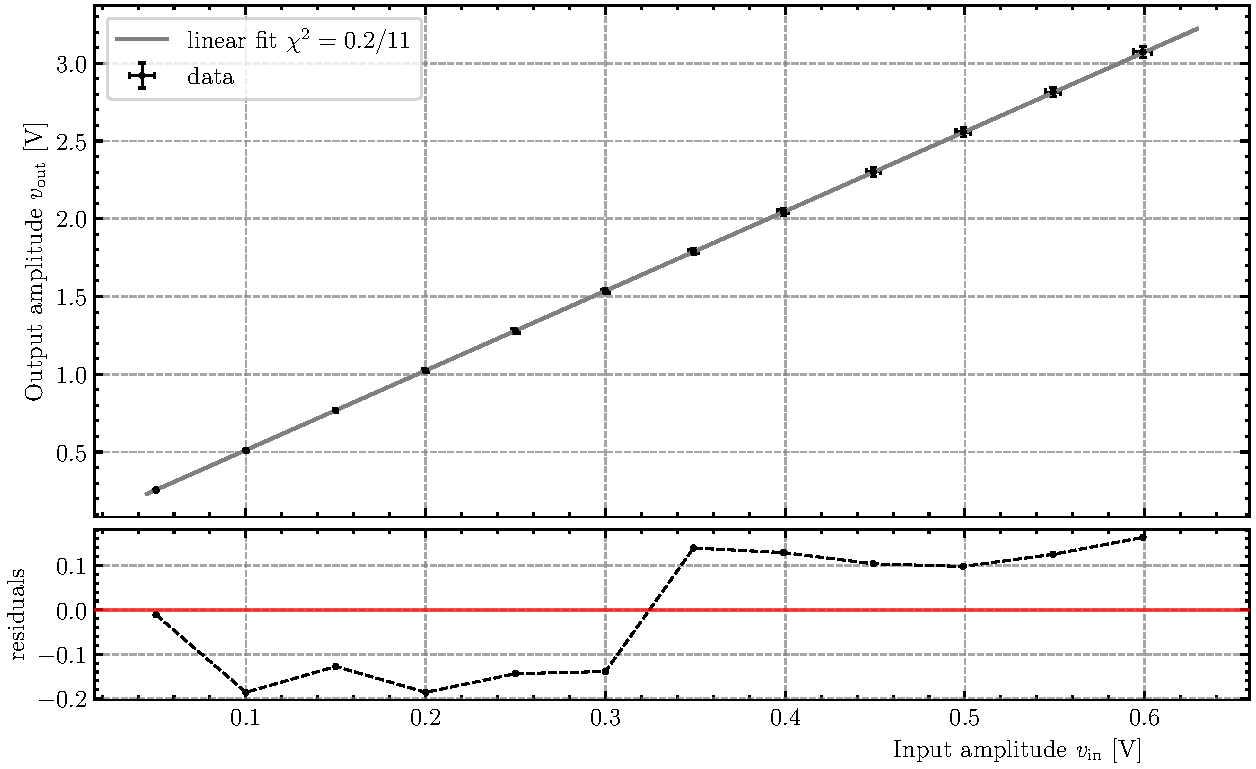
\includegraphics[scale=0.7]{gain5k1}
\caption{Fit lineare per l'andamento dell'ampiezza misurata in uscita rispetto
all'ampiezza del segnale in ingresso. \label{fig: gainfit}}
\end{figure}
Da cui troviamo i seguenti parametri per la retta di best-fit
\begin{align*}
\mathrm{intercetta} = -0.6 \pm 0.4 \; \si{m\V} \;\;\;\mathrm{pendenza} = 5.124 \pm 0.003 \;\;\;\mathrm{correlazione} 
= -0.72 \;\;\; \chi^2 = 0.2 \;\;\; d.o.f. = 10 \\
\text{coefficiente angolare/senza intercetta} = 5.120 \pm 0.002 \;\;\;
\chi^2 = 0.2 \;\;\; d.o.f. = 11
\end{align*}

Il valore atteso per il guadagno dal valore dei componenti in questa
configurazione del circuito è pari a
\[
A\ped{v, exp} = -\frac{R_2}{R_1} = - 5.13 \pm 0.12
\]
Questo è in ottimo accordo con quanto trovato sperimentalmente dalla nostra
analisi.

Per completezza riportiamo in un grafico anche le misure che non abbiamo
considerato nel fit perché oltre la regione in cui l'op-amp ha comportamento
lineare
\begin{figure}[htbp]
\centering
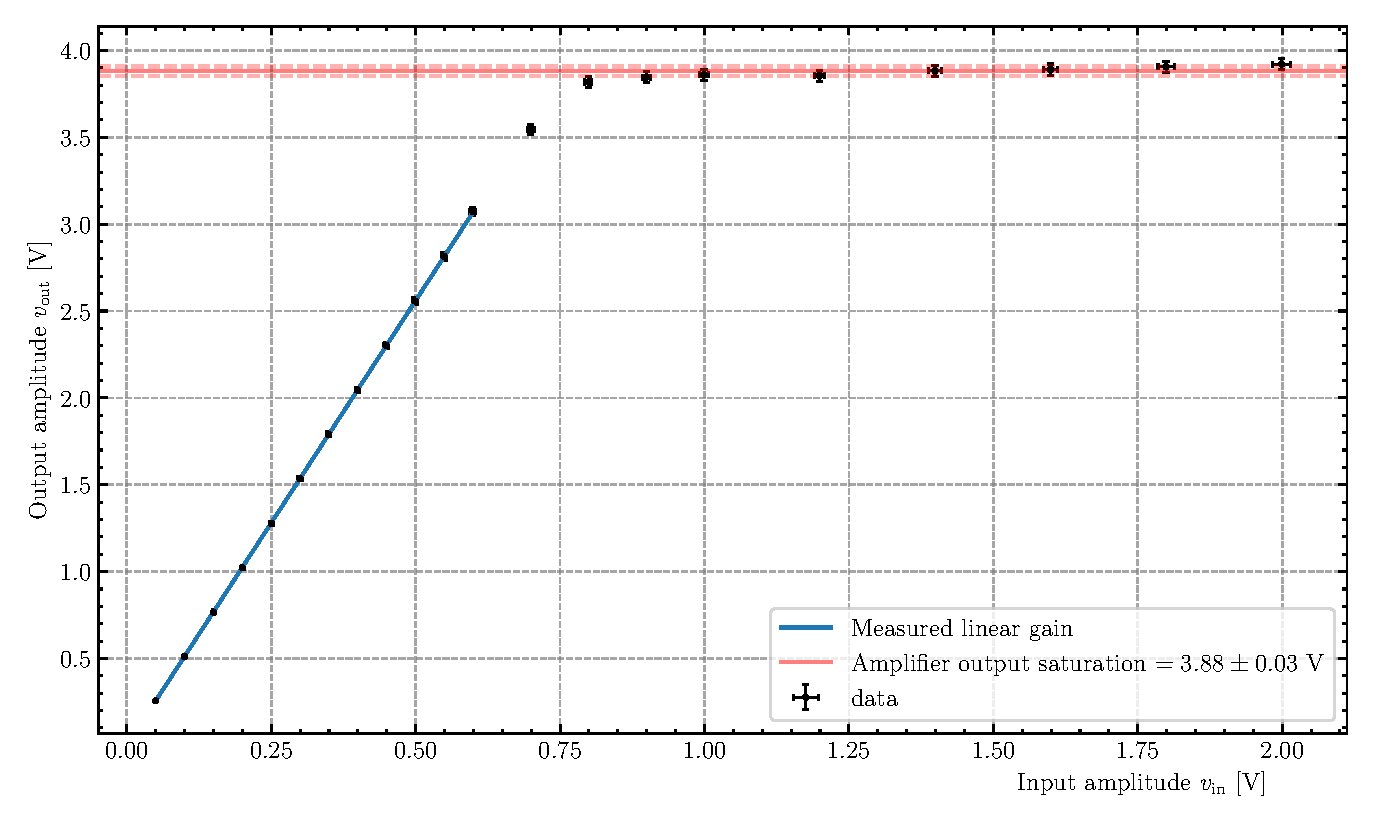
\includegraphics[scale=0.7]{gainsat}
\caption{Andamento reale dell'ampiezza del segnale in uscita al variare
dell'ampiezza del segnale in ingresso, anche oltre il regime lineare
dell'amplificatore misurati per il circuito con $R_2^a = 5.1 \; \si{k\ohm}$
\label{fig: gainsat}}
\end{figure}

\subsection{Impedenza in ingresso}
Inserendo in serie al generatore una resistenza $R_S$ dello stesso ordine di
$R\ped{in}$ attesa e misurando la tensione in uscita con o senza $R_S$ è
possibile dare un stima della resistenza in ingresso del circuito.
Detta infatti $V_1$ la tensione $V\ped{out}$ misurata senza $R_S$ e $V_2$ la
tensione misurata con $R_S$ inserita, vale la relazione:
\begin{equation}\label{eq: RS}
\frac{R_S}{R\ped{in}} = \frac{V_1}{V_2} - 1
\end{equation}
Abbiamo preso per entrambi i circuiti come $R_S$ un'altra resistenza da
$1 \pm 10\% \; \si{k\ohm}$, come quella scelta per $R_1$.

Dunque per l'amplificatore di guadagno $5.1$ abbiamo misurato
$V_1 = 1022 \pm 8 \; \si{m\V}$ e $V_2 = 512 \pm 4 \; \si{m\V}$, cioè come
resistenza in ingresso si ha:
\begin{align*}
{R\ped{in}} &= \frac{R_S}{V_1/V_2 - 1} = 0.99 \pm 0.02 \; \si{k\ohm}
\end{align*}

Mentre per l'amplificatore di guadagno $7$ si è trovato
$V_1 = 1412 \pm 8 \; \si{m\V}$ e $V_2 = 2.822 \pm 0.017 \; \si{\V}$, da cui
ricaviamo come stima della resistenza in ingresso:
\begin{align*}
{R\ped{in}} &= \frac{R_S}{V_1/V_2 - 1} = 1.00 \pm 0.02 \; \si{k\ohm}
\end{align*}

Il che risulta compatibile entro l'incertezza con il valore atteso dalla
\eqref{eq: Zin} per entrambi gli amplificatori invertenti.

\section{Risposta in frequenza e slew rate}
\subsection{Network analyzer}
Con l'aiuto dei cursori abbiamo misurato come guadagno a centro banda
per il circuito amplificatore con resistenza $R_2^a = 5.1 \; \si{k\ohm}$
$A_M = 14.18 \pm 0.09 \; \si{dB} = 5.12 \pm 0.05$.
Nel secondo caso invece ($R_2^a = 7.04 \; \si{k\ohm}$)
$A_M = 16.96 \pm 0.07 \; \si{dB} = 7.05 \pm 0.06$.
Dunque abbiamo ricavato una stima delle frequenze di taglio per i due
amplificatori invertenti dal punto in cui il guadagno diminuisce di
$-3.01 \; \si{dB}$ rispetto ad $A_M$:
\begin{align*}
f_A &= 388.0 \pm 1.1 \; \si{k\Hz} \\
f_A &= 282.8 \pm 1.6 \; \si{k\Hz}
\end{align*}

\begin{figure}[htbp]
\centering
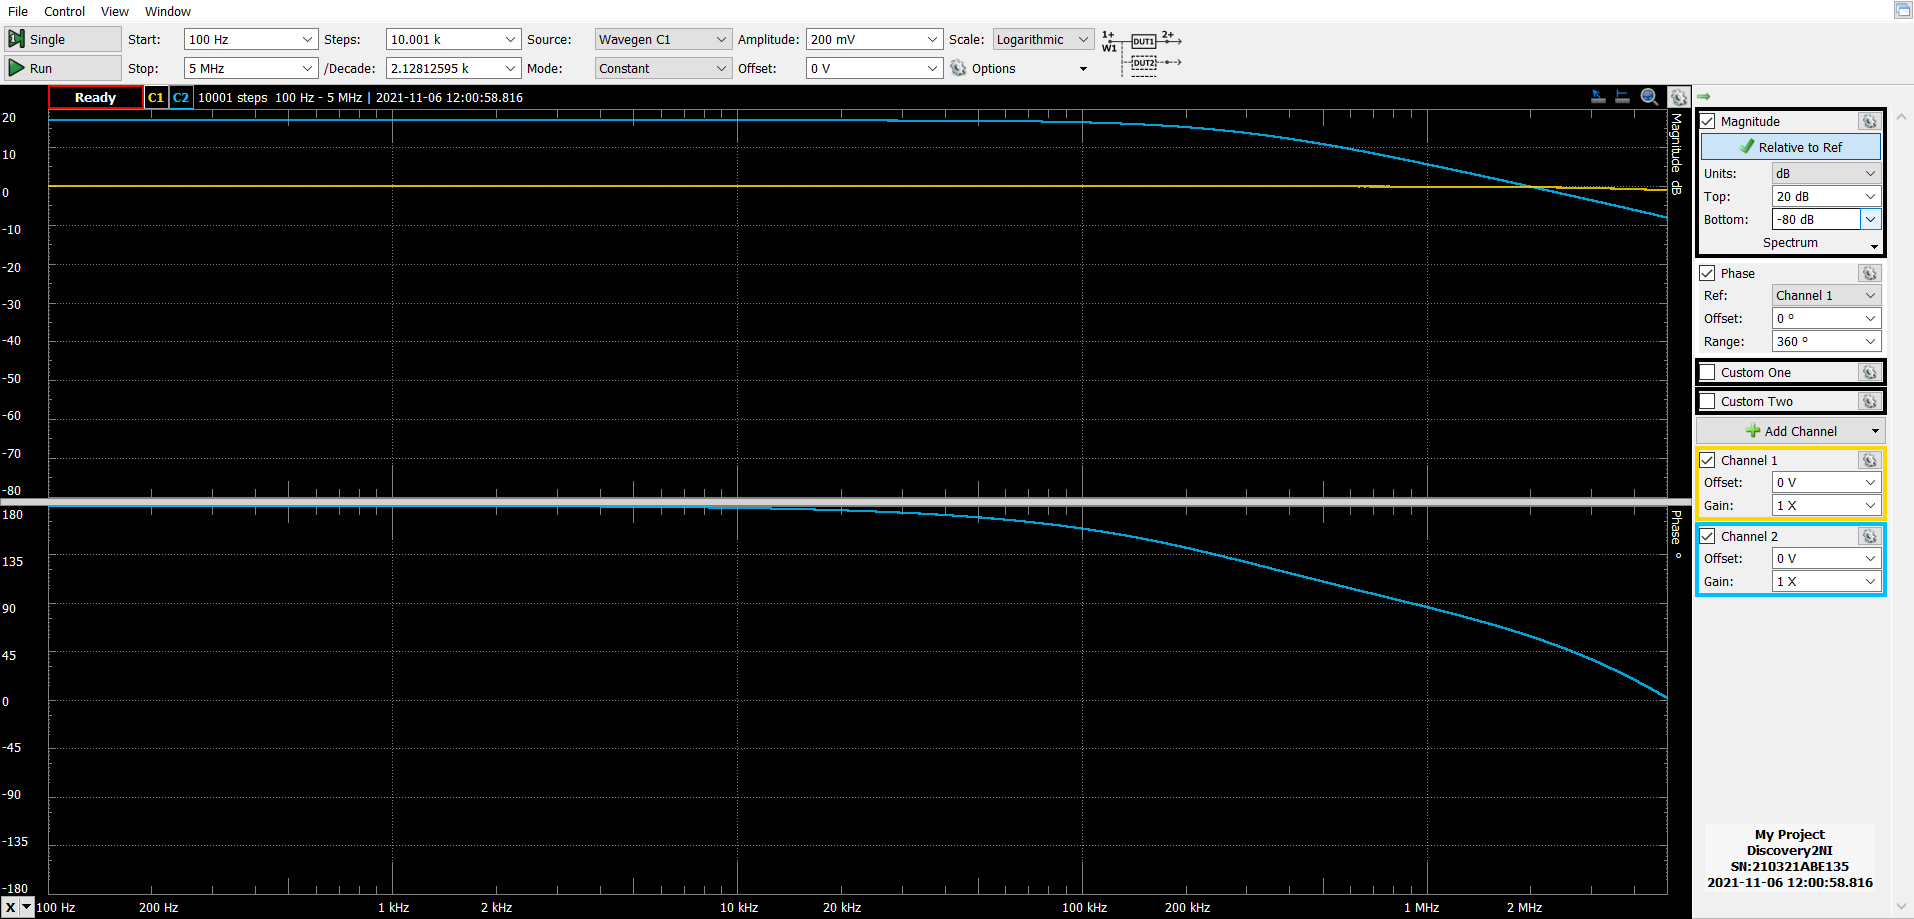
\includegraphics[scale=0.4]{opampbode}
\caption{Plot di Bode ottenuto dallo scan con Network tra $\SI{100}{\Hz}$ e
$\SI{5}{M\Hz}$ con un segnale sinusoidale in ingresso all'amplificatore
invertente di ampiezza costante $v\ped{in} = \SI{200}{m\V}$. \label{fig: invbode}}
\end{figure}

Per caratterizzare le frequenze di taglio misurate possiamo ricavare un valore
atteso con cui confrontarle a partire dal valore del prodotto banda
guadagno\footnote{Assumendo che il prodotto banda-guadagno sia costante,
come frequenza di taglio attesa in funzione del guadagno dell'amplificatore
abbiamo
$f\ped{A, exp} = \mathrm{GBW}/A_v =
\begin{cases}
\SI{4}{M\Hz} / 5.1 \approx 780 \; \si{k\Hz} \\
\SI{4}{M\Hz} / 7 \approx 570 \; \si{k\Hz}
\end{cases}$.}
(GBW) riportato nel datasheet dell'op-amp: $\SI{4}{M\Hz}$

Già dai nostri dati notiamo però come il prodotto $A_v \cdot f_H$ valga
\[
A_M \cdot f_A = 
\begin{dcases}
(5.12 \pm 0.05) \cdot (388.0 \pm 1.1) \; \si{k\Hz} =
1.99 \pm 0.03 \; \si{M\Hz} \\
%
(7.05 \pm 0.06) \cdot (282.8 \pm 1.6) \; \si{k\Hz} =
1.99 \pm 0.03 \; \si{M\Hz} \\
\end{dcases}
\]

che è circa la metà del valore tipico riportato senza incertezza per valori
di tensioni di alimentazione +15 e -15 V. Possiamo supporre che questo sia
dovuto all'aver preso come tensioni di alimentazione $V_{CC}$ e $V_{EE}$
pari a circa un terzo dei due valori tipici presi come riferimento nel
datasheet.

Quindi ci aspettiamo al più che le frequenze trovate siano prossime alla
metà dei loro valori attesi, ma assolutamente non compatibili entro
l'incertezza con il valore ottenuto dal GBW tipico.

\subsection{Misura dello slew rate}
Abbiamo inviato in ingresso all'amplificatore un'onda quadra di ampiezza
$1999 \pm 15 \; \si{m\V}$ e frequenza $1000 \pm 16 \; \si{\Hz}$, al fronte di
discesa dell'onda abbiamo trovato una rampa come segnale in uscita. Questo
permette di misurare lo slew rate dell'amplificatore direttamente dalla
pendenza della rampa.

Misurando con l'oscilloscopio di quanto sale la tensione in uscita
dall'amplificatore $\Delta V$ in un certo intervallo di tempo $\Delta t$
(presi su una porzione lineare della rampa) otteniamo una stima dello slew
rate dal loro rapporto; che rispettivamente per i circuiti con $R_2^a = 5.1$
e $7$ risulta
\begin{align*}
\mathrm{SR} = \frac{\Delta V}{\Delta t} =
\frac{6.19 \pm 0.04 \; \si{\V}}{542 \pm 10 \; \si{n\s}}
&= 11.4 \pm 0.2 \; \si{\V/\micro\s} \\
\mathrm{SR} = \frac{\Delta V}{\Delta t} =
\frac{4.10 \pm 0.03 \; \si{\V}}{354 \pm 10 \; \si{n\s}}
&= 11.6 \pm 0.2 \; \si{\V/\micro\s}  
\end{align*}

\begin{figure}[htbp]
\centering
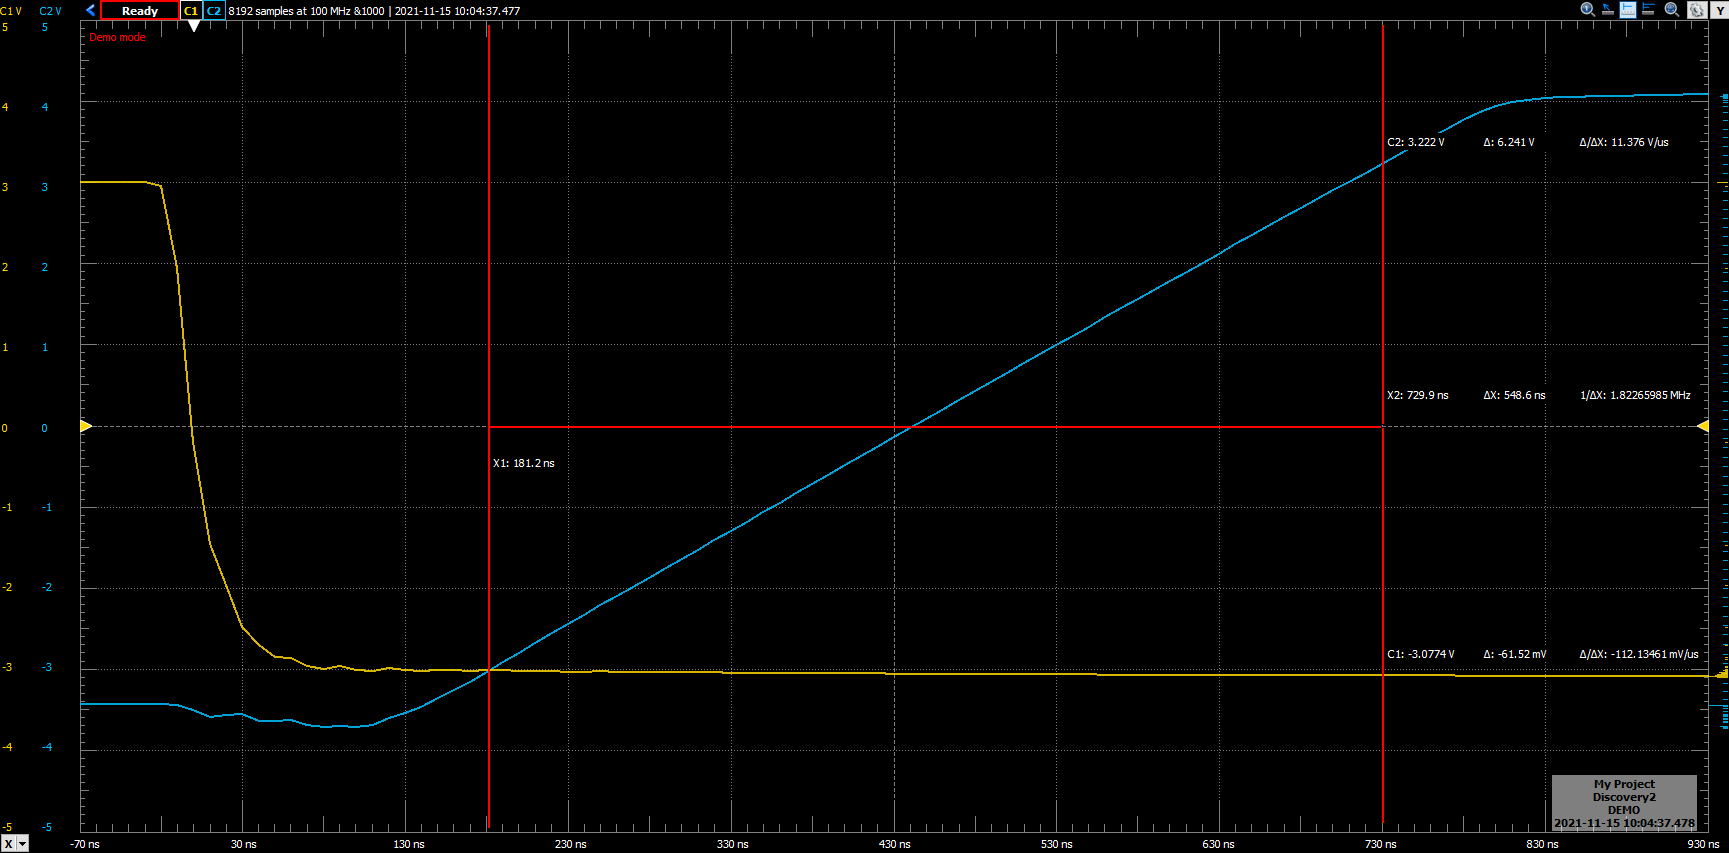
\includegraphics[scale=0.37]{slew}
\caption{La traccia della rampa in uscita dall'amplificatore visualizzata
all'oscilloscopio da cui abbiamo ottenuto la misura diretta dello slew rate.
\label{fig: slewrate}}
\end{figure}

Che di nuovo risultano sensibilmente inferiori rispetto al valore tipico
riportato nel datasheet del TL081, $SR\ped{exp} = \SI{13}{\V/\micro\s}$,
ma comunque compatibili con questo entro poco più del $10\%$. Come sopra
possiamo ipotizzare che questo sia una conseguenza della scelta (forzata
per limitazioni dell'AD2) delle tensioni di alimentazione $V_{CC}$ e $V_{EE}$
dell'op-amp minori rispetto ai valori tipici.

\section{Circuito derivatore attivo}
\subsection{Risposta in frequenza}
Partendo da una misura con i cursori del guadagno a centro banda per i
circuiti derivatori attivi
\begin{align*}
A_M &= 20.02 \pm  0.09 \; \si{dB} \\
A_M &= 20.01 \pm  0.09 \; \si{dB}
\end{align*}

possiamo ottenere una stima del valore delle frequenze di taglio a bassa
$f_c$ e ad alta frequenza $f_A$ dai punti in cui il guadagno diminuisce di un
fattore $1/\sqrt{2}$, cioè di circa $-3.01 \; \si{dB}$ rispetto ad $A_M$.
\begin{align*}
f_c &= 3.347 \pm 0.011 \; \si{k\Hz} \, ; \quad f_A = 209 \pm 2 \; \si{k\Hz} \\
f_c &= 3.15 \pm 0.04 \; \si{k\Hz} \, ; \quad f_A = 191 \pm 4 \; \si{k\Hz}
\end{align*}

\begin{figure}[htbp]
\centering
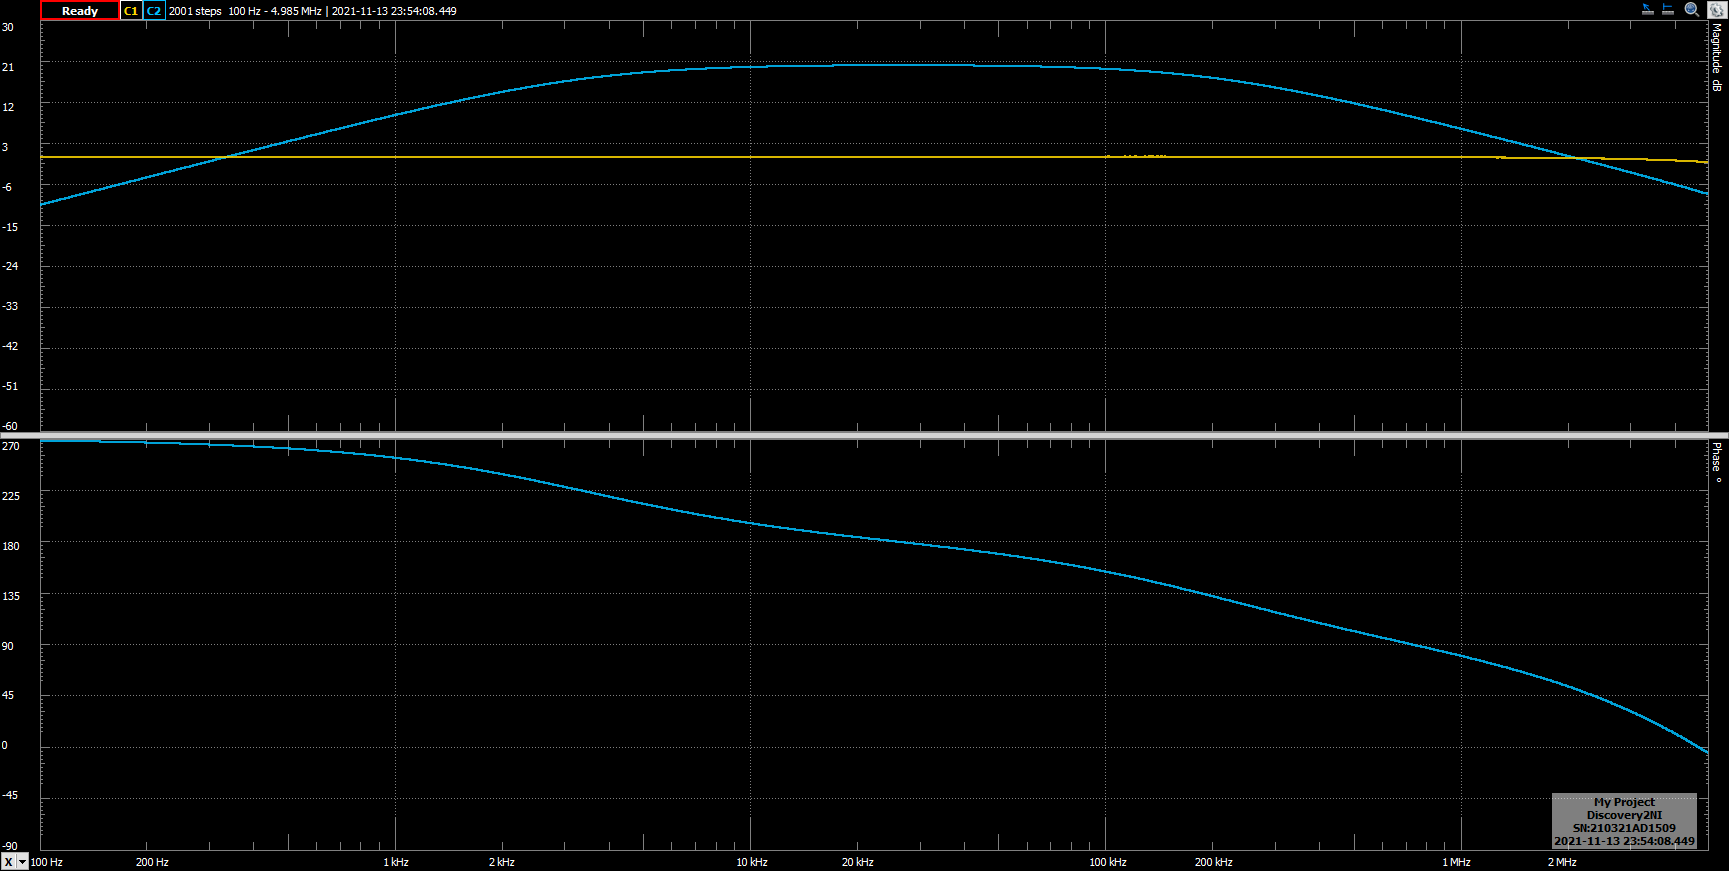
\includegraphics[scale=0.335]{hpfbode}
\caption{Plot di Bode ottenuto dallo scan con Network tra $\SI{100}{\Hz}$ e
$\SI{5}{M\Hz}$ con un segnale sinusoidale in ingresso al derivatore RC attivo
di ampiezza costante $v\ped{in} = \SI{200}{m\V}$.
\label{fig: derbode}}
\end{figure}

Notiamo come per frequenze di lavoro fino a circa $\SI{100}{k\Hz}$ il circuito si
comporta in maniera compatibile con quanto ci aspettiamo dalla funzione di
trasferimento per il nostro derivatore invertente
\begin{equation}\label{eq: hpfTfunc}
T(f) = - \frac{R_2}{Z_1(f)} = - \frac{R_2}{R_1} \frac{1}{1 - j \frac{f_c}{f}}
\end{equation}
Dunque, guadagno a centro banda
$A\ped{M, exp} = R_2/R1 = 20.01 \pm 0.10 \; \si{dB}$, pendenza
$\SI{20}{dB/decade}$ nel regime di taglio del filtro ($f \ll f_c$)
e frequenza di taglio attesa (calcolata a partire dai valori misurati dei
componenti dei circuiti studiati)
\begin{equation}\label{eq: hpfcut}
f\ped{c, exp} = \frac{1}{2\pi R_1 C} = 3.34 \pm 0.13 \; \si{k\Hz}
\end{equation}
che risulta in accordo con le nostre misure della frequenza di taglio
bassa $f_c$ del circuito derivatore.

Però, continuando ad aumentare la frequenza, come si vede dal plot di Bode in
figura \ref{fig: derbode} il circuito inizia ad avere guadagno decrescente con
pendenza $\SI{-20}{dB/decade}$ per frequenze $f \gg f_A$, come ci si aspetta
(complessivamente) per un filtro passa-banda.
 
\subsection{Risposta ad un'onda triangolare}
Si è inviato all'ingresso del filtro passa-alto un segnale triangolare di
ampiezza $v\ped{in} = 200 \pm 2 \si{m\V}$ e frequenza
$f = 100.0 \pm 1.6 \si{\Hz}$.

\begin{figure}[htbp]
\centering
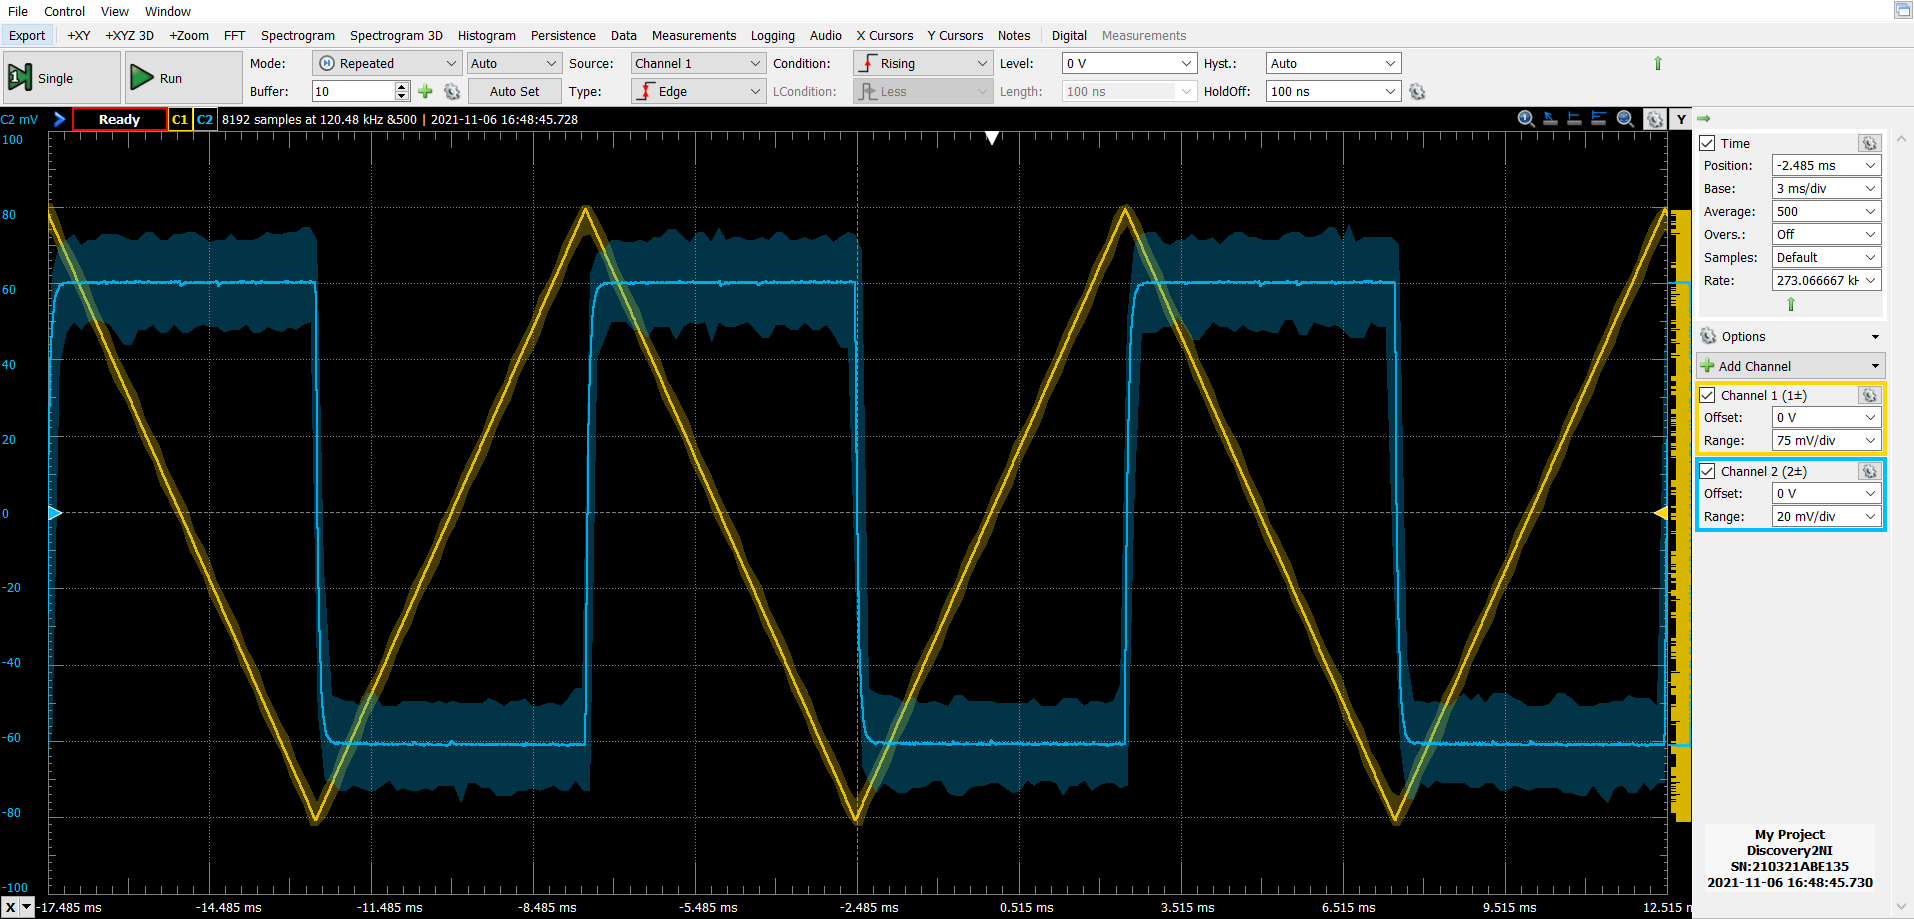
\includegraphics[scale=0.4]{derivatore}
\caption{Risposta del circuito derivatore ad un segnale triangolare di ampiezza
$\SI{200}{m\V}$ e $f = \SI{100}{\Hz}$ in ingresso. \label{fig: dertrg}}
\end{figure}

In uscita dai due circuiti abbiamo trovato un'onda quadra, come in figura
\ref{fig: dertrg} di cui riportiamo le misure di ampiezza:
\begin{align*}
v\ped{out} &= 38.0 \pm 0.3 \; \si{m\V} \\
v\ped{out} &= 40.1 \pm 0.6 \; \si{m\V} 
\end{align*}

per cui effettivamente il segnale in uscita assume la forma della derivata
del segnale in ingresso, con ampiezza ridotta di
$A_v = \nicefrac{v\ped{out}}{v\ped{in}} = 0.195 \pm 0.005 $

Per frequenze $f \ll f_c$ il filtro è in regime di taglio, per cui si comporta
come un derivatore, dunque la forma d'onda in uscita è un'onda quadra di
ampiezza sempre minore al diminuire della frequenza.

Per frequenze $f_c \ll f \ll f_A$ come ci si aspetta, la forma d'onda in uscita
rimane visivamente inalterata rispetto all'onda triangolare in ingresso,
che risulta però amplificata in ampiezza di un fattore $A_M \sim 10$.

Nel regime intermedio $f \sim f_c$ all'uscita del filtro RC osserviamo un'onda
"a pinna di squalo" caratteristica della carica e della scarica del
condensatore con cui abbiamo costruito il nostro filtro passa-alto.
\begin{figure}[htbp]
\centering
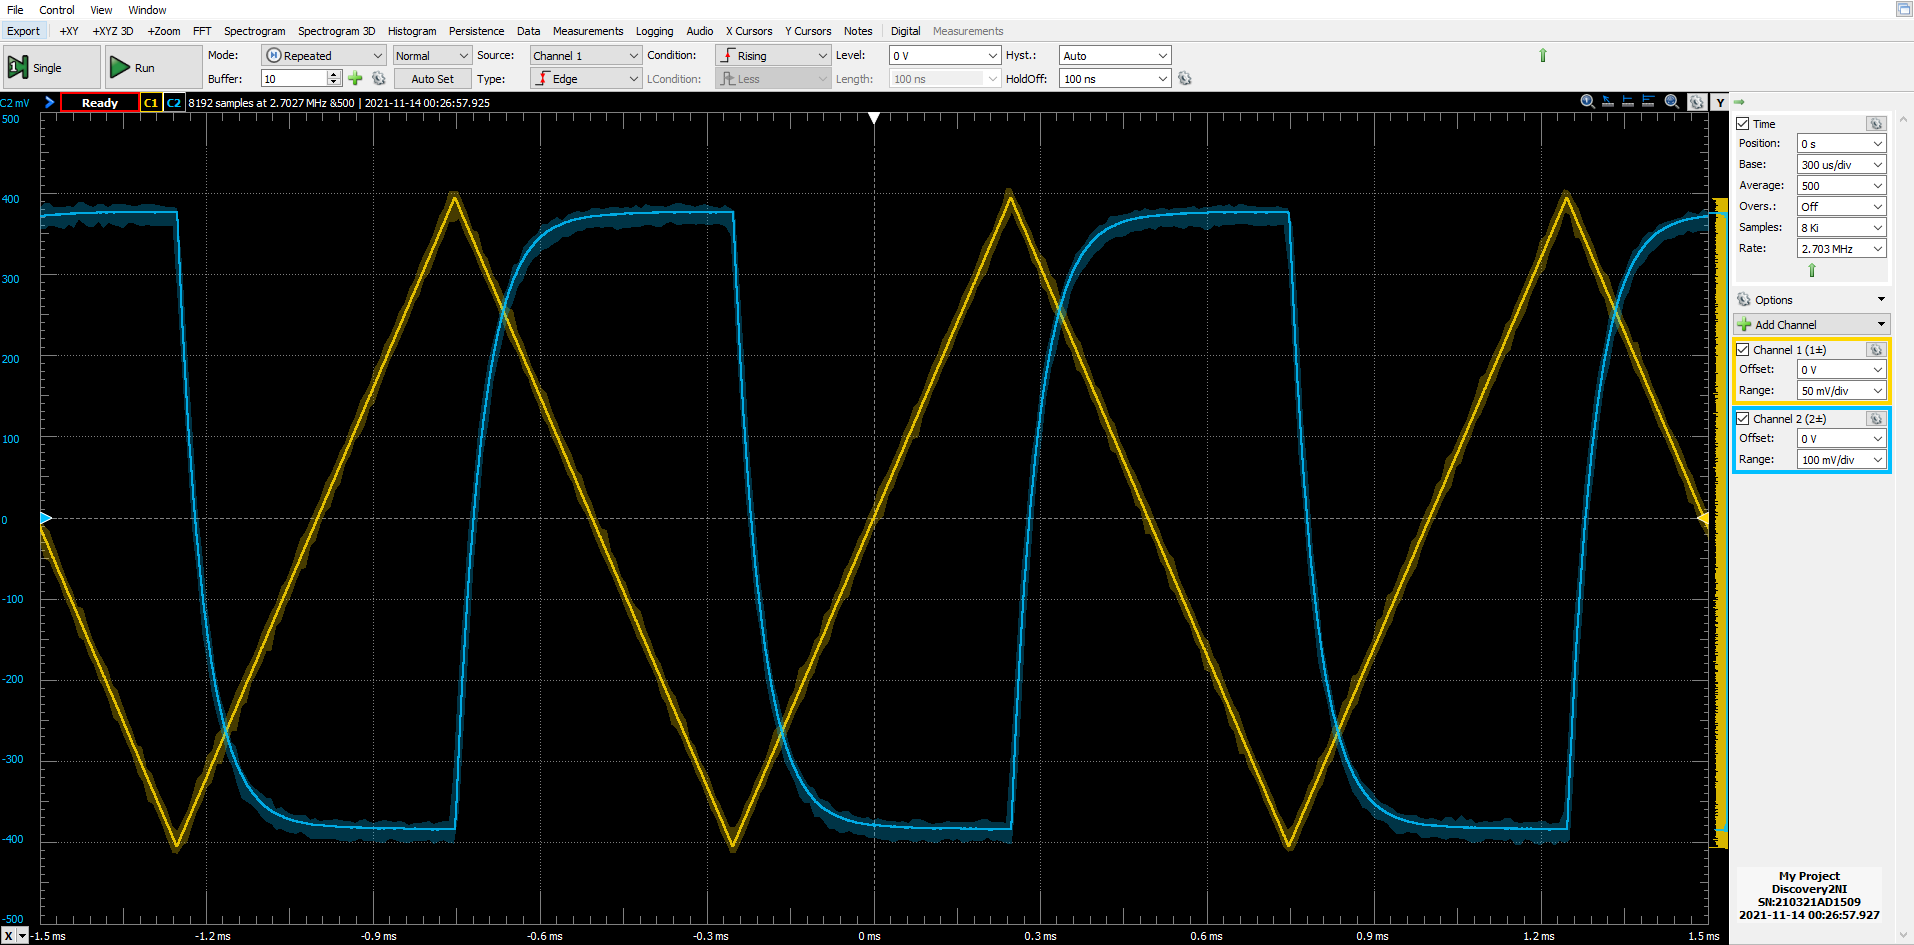
\includegraphics[scale=0.335]{derfin}
\caption{Onda a pinna di squalo in risposta ad un triangolo di ampiezza
$200 \pm 2 \; \si{m\V}$ e $f = 1000 \pm 16 \; \si{Hz}$ in ingresso al
circuito derivatore. \label{fig: derfin}}
\end{figure}

Per frequenze $f \gg f_A$ il filtro torna in regime di taglio, ma ora si
comporta grosso modo come un integratore, infatti la forma d'onda in uscita è
costituita da una serie di parabole con concavità rivolte verso l'alto e verso
il basso con ampiezza sempre minore all'aumentare della frequenza.
\begin{figure}[htbp]
\centering
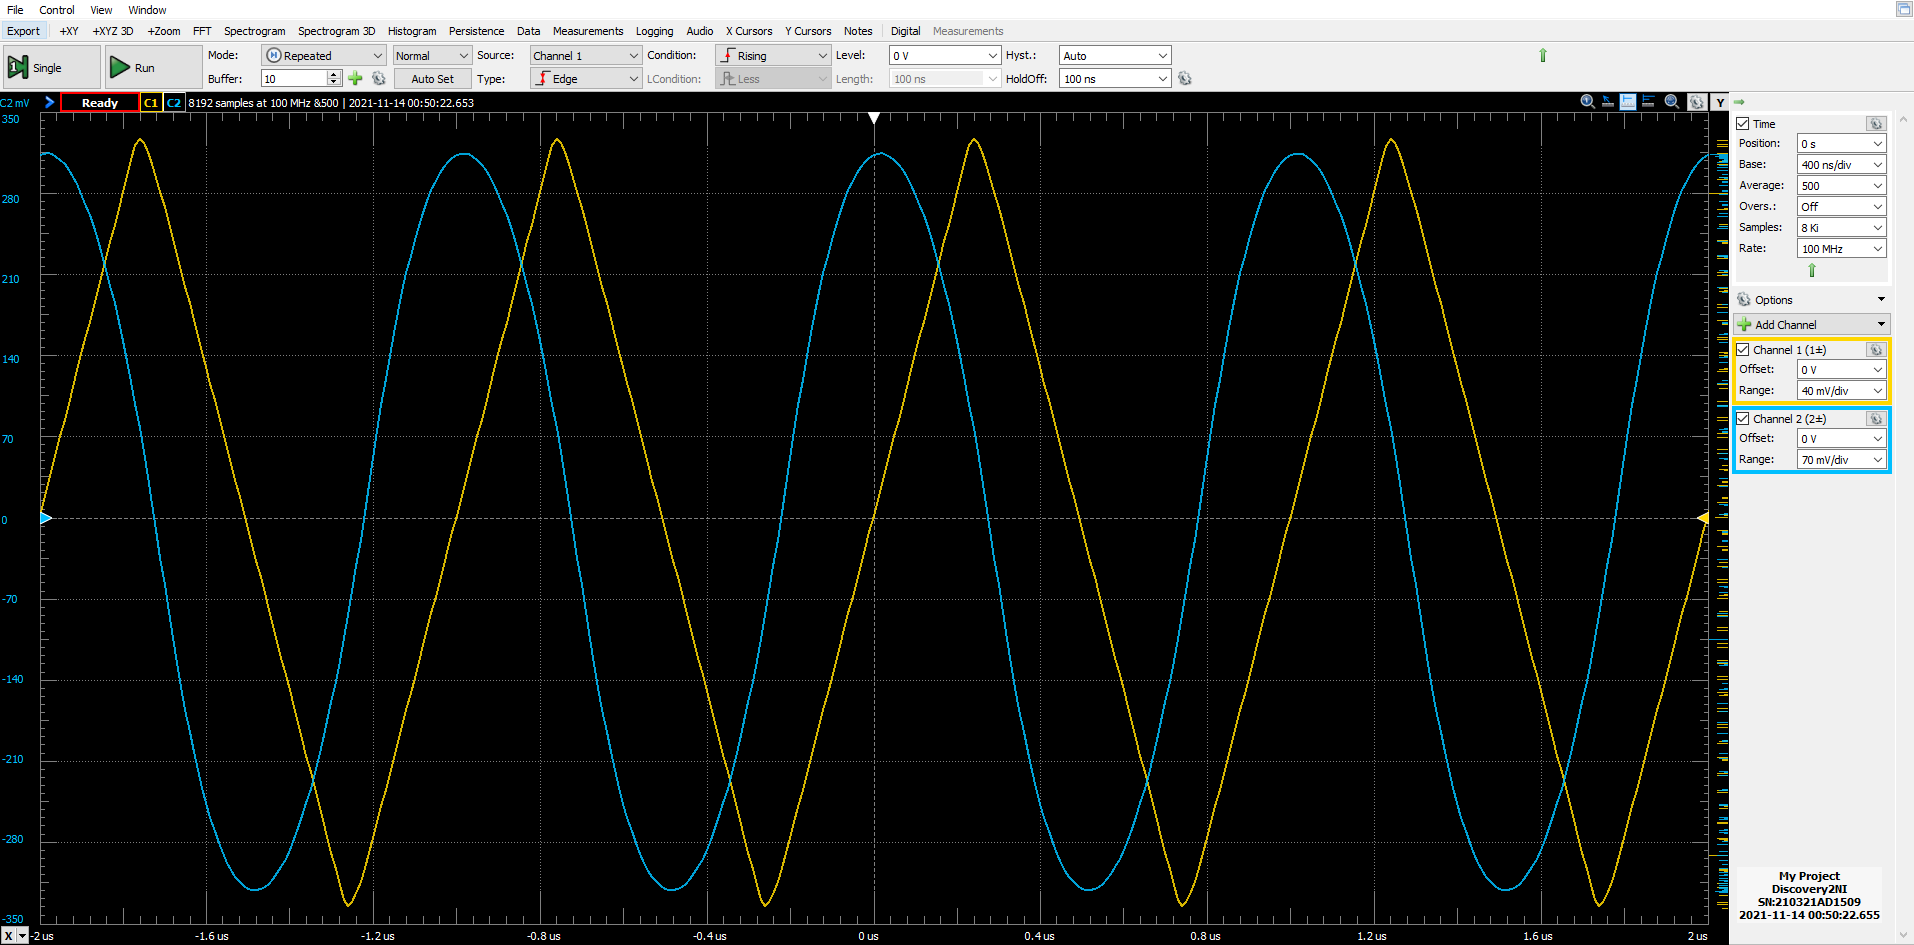
\includegraphics[scale=0.335]{derpar}
\caption{Parabole con concavità alternanti in risposta ad un triangolo di
ampiezza $200 \pm 2 \; \si{m\V}$ e $f = 1.00 \pm 0.02 \; \si{M\Hz}$ in ingresso
al circuito derivatore. \label{fig: derpar}}
\end{figure}

\subsection{Confronto con i valori attesi}
Assumendo che il prodotto banda-guadagno rimanga costante possiamo verificare
che la frequenza di taglio alta sia dovuta alla limitazione di banda
dell'op-amp reale, confrontandola con quella attesa per il guadagno $A_M$ del
passa-alto attivo
$f\ped{A, exp} = \mathrm{GBW}/A_M
= (1.99 \pm 0.02 \; \si{M\Hz})/(10.00 \pm 0.10) = 199 \pm 2 \; \si{k\Hz}$.
Questo è compatibile entro il $5\%$ con il valore di frequenza $f_A$ misurato,
ma preferiamo controllare che la frequenza di taglio alta del passa-banda
corrisponda proprio a quella di un amplificatore con guadagno 10 come ulteriore
conferma.

Quindi, una volta realizzato un nuovo amplificatore invertente con la
stessa resistenza $R_2$ del filtro (i.e. scollegando il condensatore)
misuriamo dal plot di Bode la frequenza di taglio con i cursori
$f_H = 207.8 \pm 1.3 \; \si{k\Hz}$
\begin{figure}[htbp]
\centering
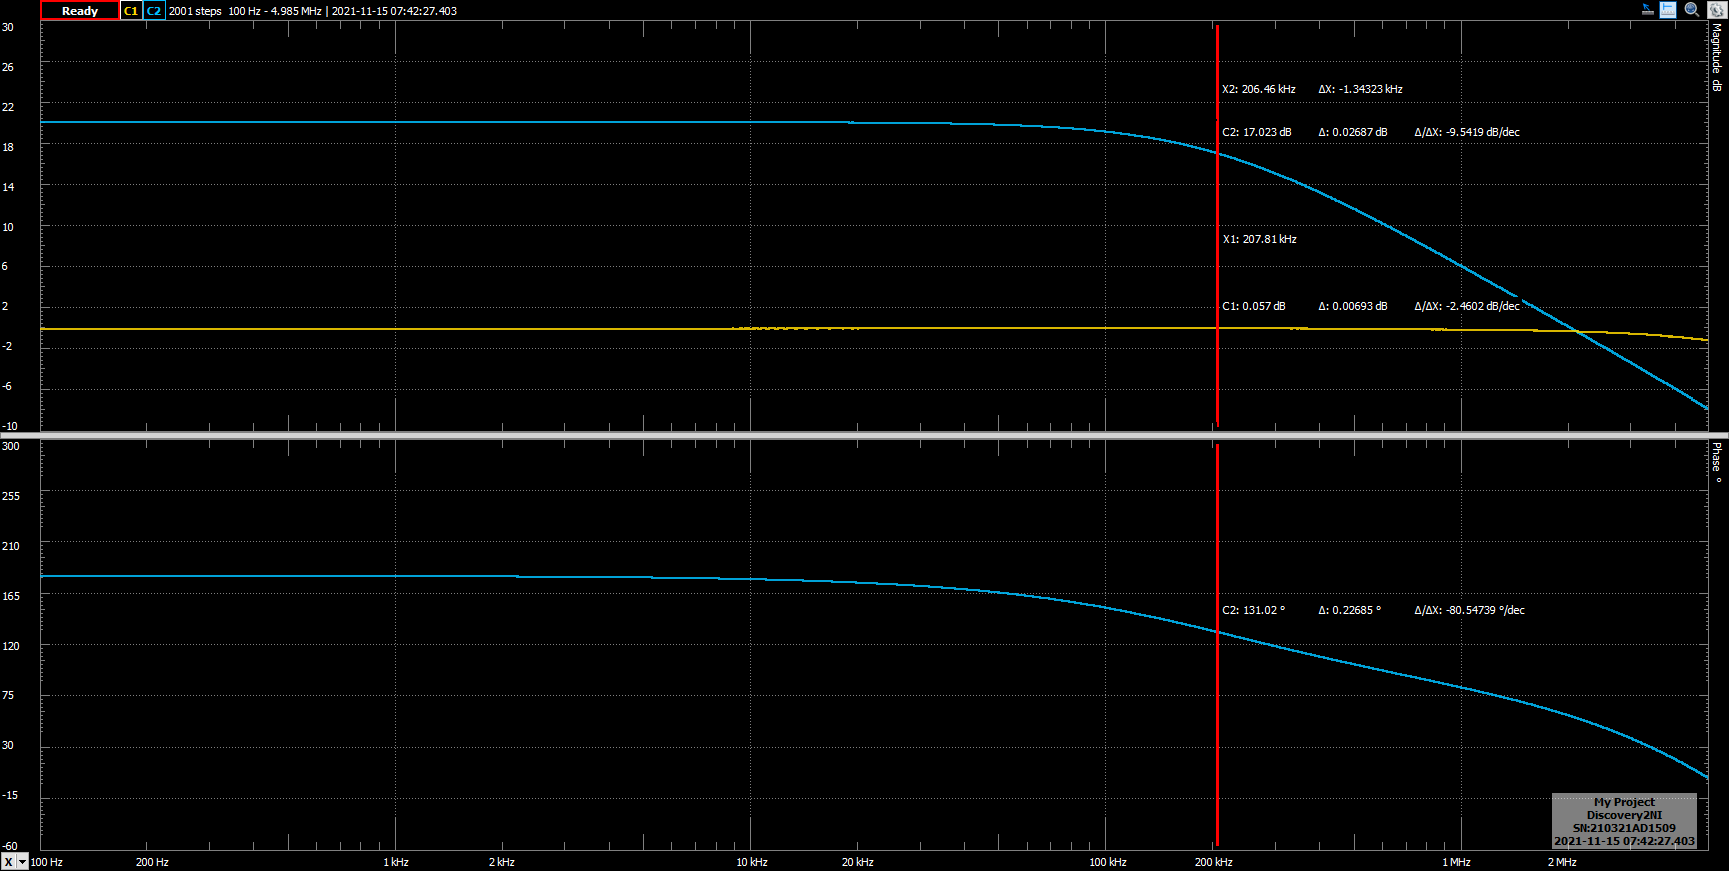
\includegraphics[scale=0.36]{ampinv10}
\caption{Plot di Bode ottenuto dallo scan con Network tra $\SI{100}{\Hz}$ e
$\SI{5}{M\Hz}$ con un segnale sinusoidale in ingresso all'amplificatore
invertente (con $R_2^f=10$) di ampiezza costante $v\ped{in} = \SI{200}{m\V}$.
\label{fig: ampinv10}}
\end{figure}

Questa è compatibile entro l'incertezza con $f_A$ misurata per il derivatore,
per cui possiamo dire che il circuito si comporta come un passa-banda per via
del limite in frequenza dell'op-amp, il quale determina la frequenza di taglio
alta del filtro.

Detta $V_{0} = v\ped{in} $ l'ampiezza del segnale in ingresso, la componente
principale nello sviluppo in serie di Fourier dell'onda triangolare ha ampiezza 
$\frac{8}{\pi^2} V_{0} $ e frequenza pari a quella della portante $f$.
Dalla funzione di trasferimento \eqref{eq: hpfTfunc} sviluppata per frequenze
$f \ll f_c$, la componente principale dell'onda in uscita ha ampiezza
$\frac{8}{\pi^2} V_{0} 2\pi R_2 C f $. Pertanto ci aspettiamo che l'onda
triangolare in uscita abbia ampiezza riscalata di un fattore $\pi/4$, che è
il reciproco del fattore di ampiezza raccolto da ogni coefficiente dello
sviluppo in serie di Fourier di un'onda quadra:
\[
v\ped{out, exp} = \frac{8}{\pi^{2}} V\ped{in} 2 \pi R_{2} C f \frac{\pi}{4} =
4 v\ped{in} R_{2} C f = 37.3 \pm 1.5 \; \si{m\V}
\]
che risulta compatibile con l'ampiezza del segnale misurato in uscita.

Senza la resistenza $R_1$ il circuito (in approssimazione di ground virtuale)
avrebbe come funzione di trasferimento
\[
T(\omega) = - j \omega R_2 C \implies
\abs{T(f)} = A(f) =  - 2\pi f R_2 C
\]
Dunque un guadagno corrispondente nel diagramma di Bode ad una retta di
pendenza costante $\SI{20}{\deci\bel/decade}$.
Questo implica una divergenza del segnale in uscita per alte frequenze, la
quale porterebbe l'op-amp in regime non lineare di saturazione.
In altre parole avremmo un derivatore in cui però non abbiamo controllo sulla
frequenza di taglio e con segnale in uscita affetto da clipping ad alte
frequenze.

La resistenza in serie al condensatore ci permette in primo luogo di
stabilire la frequenza di taglio come in equazione \eqref{eq: hpfcut} e,
in secondo, di limitare il guadagno massimo a $R_2/R_1$;
indipendentemente dal valore dei parametri di costruzione dell'op-amp.

%=======================
\section{Circuito integratore attivo}
\subsection{Risposta in frequenza}
Di nuovo utilizzando i cursori abbiamo misurato come guadagno a centro banda
per i circuiti integratori
\begin{align*}
A_M &= 19.92 \pm 0.09 \; \si{dB} \\
A_M &= 19.95 \pm 0.09 \; \si{dB}
\end{align*}

Dunque abbiamo ricavato le nostre stime per le frequenze di taglio del filtro
passa-basso dal punto in cui il guadagno diminuisce di $-3.01 \; \si{dB}$
rispetto ad $A_M$:
\begin{align*}
f_c &= 335 \pm 2 \; \si{\Hz} \\
f_c &= 317.4 \pm 0.5 \; \si{\Hz} \\
\end{align*}

\begin{figure}[htbp]
\centering
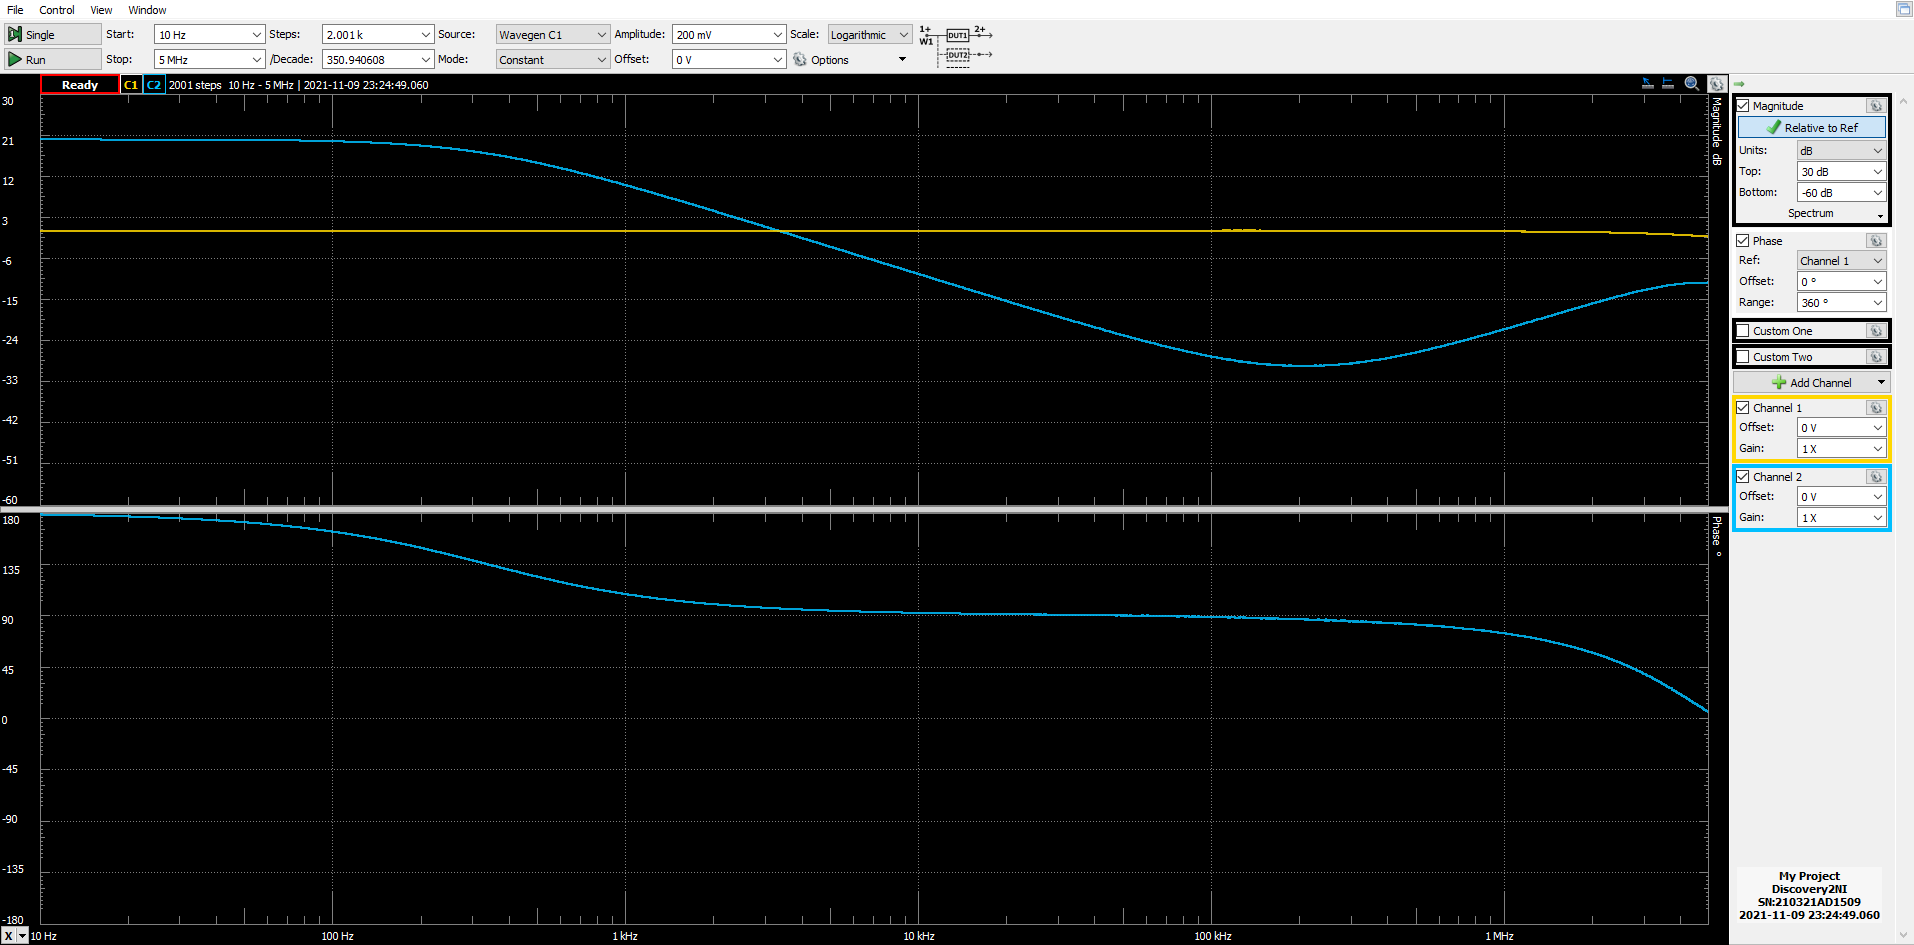
\includegraphics[scale=0.335]{lpfbode}
\caption{Plot di Bode ottenuto dallo scan con Network tra $\SI{10}{\Hz}$ e
$\SI{5}{M\Hz}$ con un segnale sinusoidale in ingresso all'integratore RC
attivo di ampiezza costante $v\ped{in} = \SI{200}{m\V}$.
\label{fig: intbode}}
\end{figure}

La frequenza di taglio attesa per il filtro passa-basso calcolata a partire
dai valori misurati dei componenti dei circuiti risulta
\begin{equation}\label{eq: lpfcut}
f\ped{c, exp} = \frac{1}{2\pi R_2 C} = 334 \pm 13 \; \si{\Hz}
\end{equation}
che risulta in ottimo accordo con le nostre misure della frequenza di taglio
bassa $f_c$ del circuito integratore.

Notiamo come per frequenze di lavoro fino a circa $\SI{100}{k\Hz}$ il circuito
si comporta in maniera compatibile con quanto ci aspettiamo dalla funzione di
trasferimento per il nostro integratore invertente
\begin{equation}\label{eq: lpfTfunc}
T(f) = \frac{Z_2(f)}{R_1} = - \frac{R_2}{R_1} \frac{1}{1 + j \frac{f}{f_c}}
\end{equation}
Ovvero, guadagno a centro banda
$A\ped{M, exp} = R_2/R1 = 20.01 \pm 0.10 \; \si{dB}$ e pendenza
$\SI{-20}{dB/decade}$ nel regime di taglio del filtro ($f \gg f_c$).

Per frequenze maggiori dal plot di Bode in figura \ref{fig: intbode} vediamo
che il guadagno assume un minimo a circa $-29.5 \pm 0.5 \; \si{dB}$ per
una frequenza $f = 186 \pm 2 \; \si{k\Hz}$ e inverte il suo andamento fino
ad assumere pendenza leggermente inferiore a $\SI{20}{dB/decade}$, in maniera
simile a quanto ci si aspetta per il passaggio da uno zero di ordine 2
nella funzione di trasferimento del sistema.

Risulta difficile da valutare se questo sia dovuto ad accoppiamenti capacitivi
fra basetta, fili e componenti passivi del circuito, alle capacità parassite
dentro il TL081 o ad entrambi, che non stiamo considerando nel nostro modello.

Senza la resistenza $R_2$ il circuito (in approssimazione di ground virtuale)
avrebbe come funzione di trasferimento
\[
T(\omega) = - \frac{1}{j \omega R_1 C} \implies
\abs{T(f)} = A(f) = \frac{1}{2\pi f R_1 C}
\]
Dunque un guadagno corrispondente nel diagramma di Bode ad una retta di
pendenza costante $\SI{-20}{\deci\bel/decade}$.
Questo implica una divergenza del segnale in uscita per basse frequenze, la
quale porterebbe l'op-amp in regime non lineare di saturazione.
Cioè avremmo un integratore in cui però non abbiamo controllo sulla
frequenza di taglio e con segnale in uscita affetto da clipping a basse
frequenze.

La resistenza in parallelo al condensatore ci permette in primo luogo di
stabilire la frequenza di taglio come in equazione \eqref{eq: lpfcut} e,
in secondo, di limitare il guadagno massimo a $R_2/R_1$;
indipendentemente dal valore dei parametri di costruzione dell'op-amp.

\subsection{Risposta ad un'onda quadra @ 10 kHz}
Si è inviato all'ingresso del filtro passa-basso un'onda quadra di
ampiezza $v\ped{in} = 200 \pm 2 \; \si{m\V}$ e frequenza
$10.02 \pm 0.12 \; \si{k\Hz}$.

\begin{figure}[htbp]
\centering
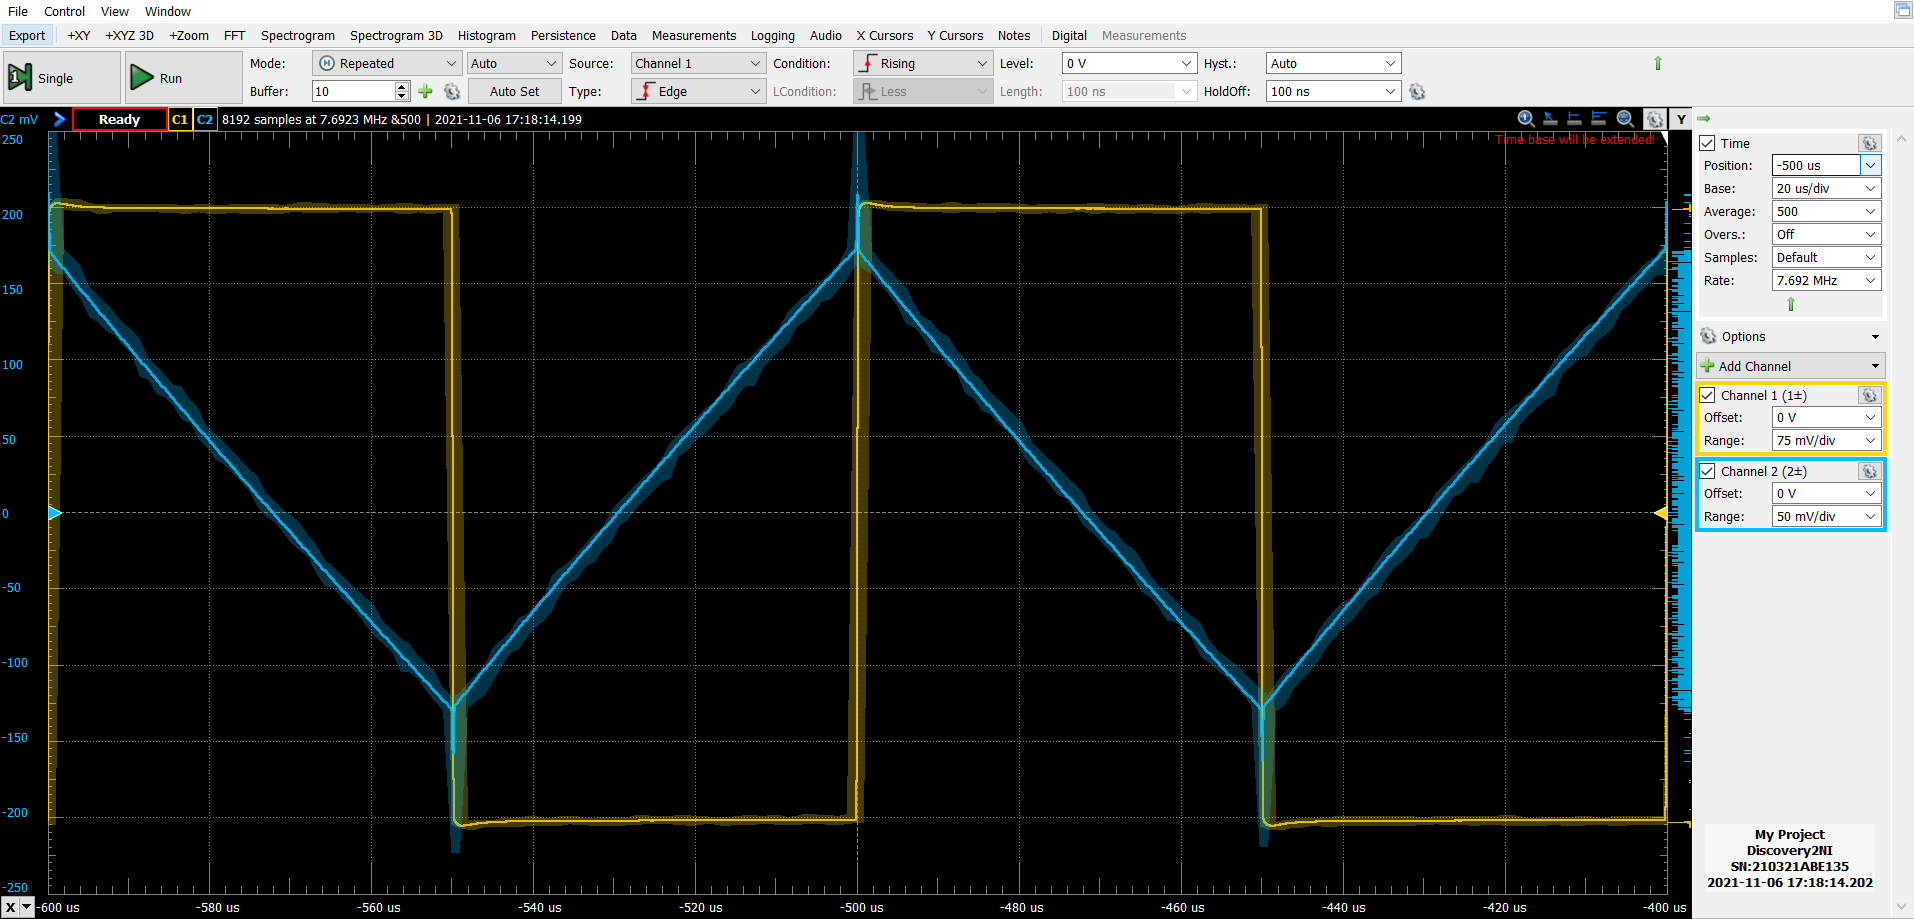
\includegraphics[scale=0.42]{integratore}
\caption{Risposta del circuito integratore ad un'onda quadra di ampiezza
$\SI{200}{m\V}$ e $f = \SI{10}{k\Hz}$ in ingresso. \label{fig: intsqw}}
\end{figure}

In uscita abbiamo trovato un'onda triangolare, come si vede in figura
\ref{fig: intsqw} di cui riportiamo le misure di ampiezza:
\begin{align*}
v\ped{out} = 107.3 \pm 1.3 \; \si{m\V} \, ; \quad
A_v = \frac{v\ped{out}}{v\ped{in}} = 0.537 \pm 0.008 \\
v\ped{out} = 100.5 \pm 1.2 \; \si{m\V} \, ; \quad
A_v = \frac{v\ped{out}}{v\ped{in}} = 0.503 \pm 0.007
\end{align*}
per cui effettivamente il segnale in uscita è la forma d'onda integrale
di quella in ingresso, con ampiezza ridotta di circa la metà.

Per frequenze $f \ll f_c$ come è ragionevole aspettarsi, la forma d'onda in
uscita non è apprezzabilmente cambiata rispetto all'onda quadra in ingresso,
ma risulta soltanto amplificata in ampiezza di un fattore $A_M \sim 10$.

Per frequenze $f \gg f_c$ il filtro è in regime di taglio, per cui si comporta
come un integratore, dunque la forma d'onda in uscita è un'onda triangolare di
ampiezza sempre minore al crescere della frequenza.

Nel regime intermedio $f \sim f_c$ all'uscita del filtro RC osserviamo un'onda
"a pinna di squalo" che corrispondono alle curve di carica e scarica del
condensatore al passaggio da basso ad alto e viceversa dell'onda quadra in
ingresso.
\begin{figure}[htbp]
\centering
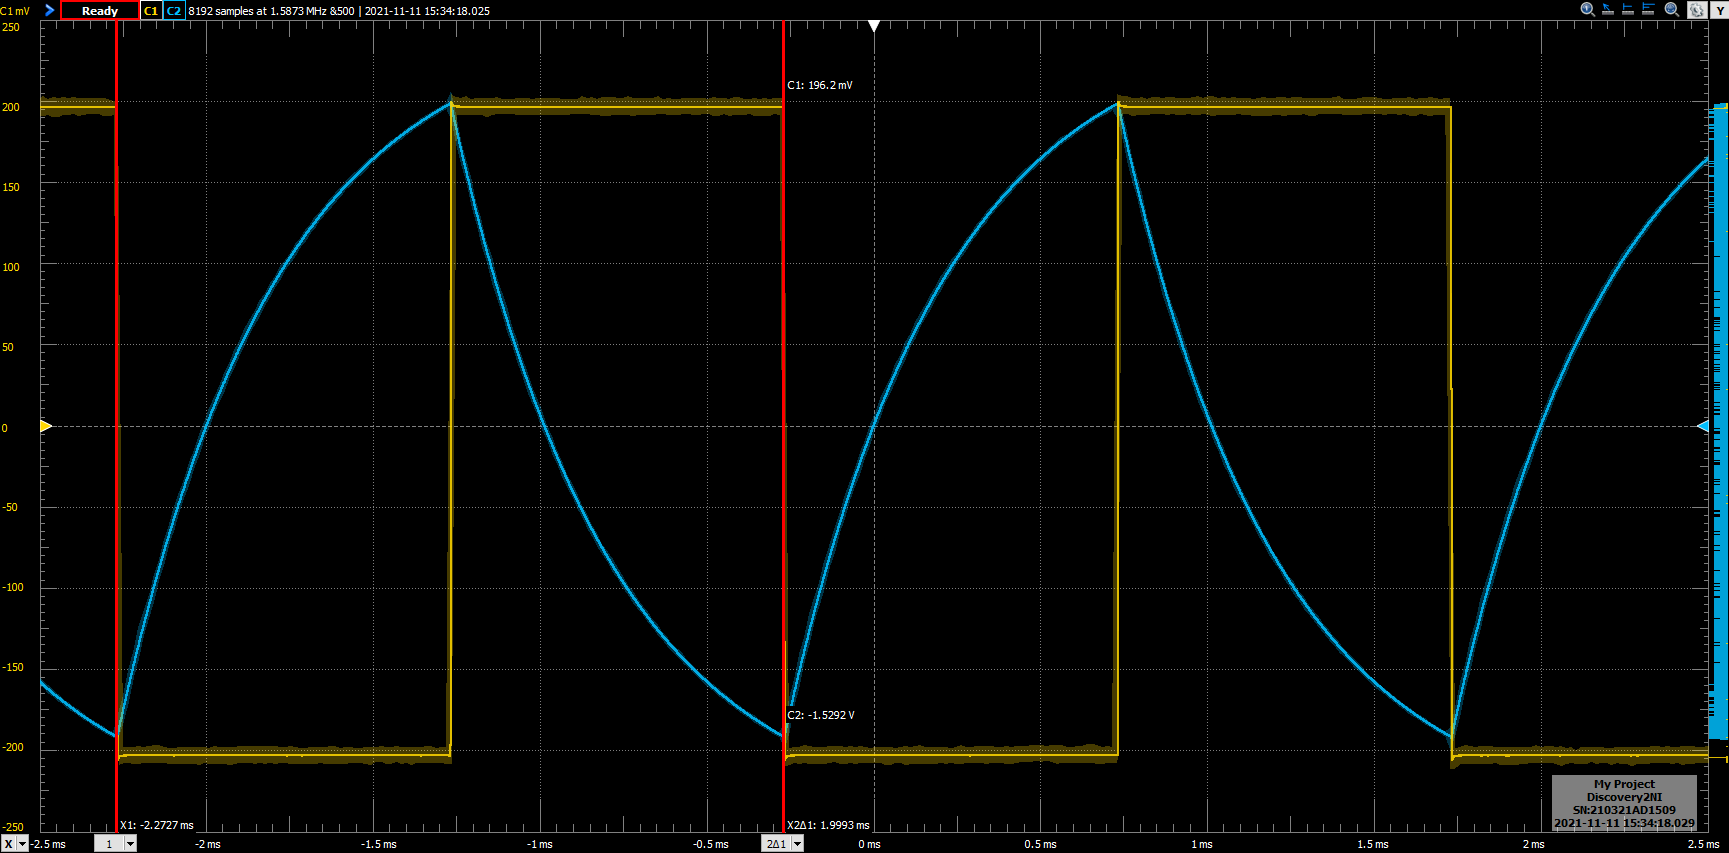
\includegraphics[scale=0.335]{intfin}
\caption{Onda a pinna di squalo in risposta ad un'onda quadra di ampiezza
$\SI{200}{m\V}$ e $f = 500 \pm 6 \; \si{Hz}$ in ingresso al circuito
integratore. \label{fig: intfin}}
\end{figure}

In corrispondenza dei fronti di salita/discesa dell'onda quadra in ingresso
osserviamo dei picchi di tensione in uscita, che alterano apprezzabilmente
la forma d'onda triangolare. La loro presenza potrebbe essere dovuta al fatto
che l'approssimazione di ground virtuale non sia verificata in questo caso,
per cui si determina una caduta di tensione sulla resistenza interna $R_{in}$
dell'op-amp che quindi devia dal comportamento atteso.

Ripercorrendo al contrario il ragionamento di prima, se $V_0 = v\ped{in}$ è
l'ampiezza dell'onda quadra in ingresso, la sua componente principale nello
sviluppo in serie di Fourier ha ampiezza $\frac{4}{\pi} V_0$ e la stessa
frequenza della portante scelta con Wavegen $f_0 = f$.
Applicando la funzione di trasferimento \eqref{eq: lpfTfunc} approssimata per
frequenze $f \gg f_c$, la componente principale del segnale in uscita ha
ampiezza $\frac{4}{\pi} V_0 / 2\pi R_1 C f$. Finalmente ci aspettiamo che
l'onda triangolare in uscita abbia ampiezza scalata di un ulteriore fattore
$\pi^2/8$, dato dal suo sviluppo in serie:
\[
v\ped{out, exp} = \frac{4}{\pi} \frac{v\ped{in}}{2 \pi R_1 C f} \frac{\pi^2}{8} =
\frac{v\ped{in}}{4 R_1 C f} = 107 \pm 4 \; \si{m\V}
\]
che risulta compatibile con l'ampiezza del segnale misurato in uscita.

\section{Circuito amplificatore non invertente}
\subsection{Risposta in frequenza}
\begin{figure}[htbp]
\centering
%\includegraphics[scale=0.35]{ninvbode}
\caption{Plot di Bode ottenuto dallo scan con Network tra $\SI{100}{\Hz}$ e
$\SI{5}{M\Hz}$ con un segnale sinusoidale in ingresso all'amplificatore
non-invertente di ampiezza costante $v\ped{in} = \SI{200}{m\V}$.
\label{fig: ampbode}}
\end{figure}

\subsection{Misure di guadagno e frequenza di taglio}
Partendo da una misura con i cursori del guadagno a centro banda,
$A_V = 19.65 \pm 0.05 \; \si{dB} = 9.65 \pm 0.08$, possiamo ottenere una stima del valore
delle frequenze di taglio a bassa $f_L$ e ad alta frequenza $f_H$ dai punti
in cui il guadagno diminuisce di un fattore $1/\sqrt{2}$, cioè di circa
$-3.01 \; \si{dB}$ rispetto ad $A_V$.
\begin{align*}
f_L &= 80.77 \pm 0.12 \; \si{\Hz}\\
f_H &= 646.1 \pm 0.5 \; \si{k\Hz}
\end{align*}
\iffalse
Una volta inserito il ramo in parallelo a $R_E$, dalla formula per il guadagno
atteso otteniamo
\[
A_v = -\frac{R_C}{\abs{Z_E}} =
- \frac{R_C}{R_E \; \lvert \rvert \; \left(R\ped{es} + \abs{1/j\omega C_E}
\right)} =
- R_C \abs{\frac{1}{R_E} + \frac{1}{R\ped{es} + 1/\omega C_E}}
\]

Visto che abbiamo scelto $C_E \gg C\ped{in} \sim C\ped{out}$, alla frequenza
di lavoro $f = \SI{10}{k\Hz}$ possiamo considerare trascurabile l'impedenza
del condensatore $\abs{Z_{C_E}} = \dfrac{1}{2\pi f C_E} \approx 0.1 \si{\ohm}
\ll R\ped{es}$, per cui in buona approssimazione ci aspettiamo
\[
\abs{A_v} \approx
\frac{R_C}{R_E \; \lvert \rvert \; R\ped{es}} =
R_C \abs{\frac{1}{R_E} + \frac{1}{R\ped{es}}} \approx
\frac{R_C}{R\ped{es}} = 110 \pm 1
\]

Questo però assumendo che l'impedenza del transistor sia trascurabile rispetto
a $Z_E$, o meglio $\abs{Z_E} \gg \dfrac{h_{ie}}{h_{fe}}$
\begin{align*}
\abs{Z_E} &= \abs{\frac{1}{R_E} + \frac{1}{R\ped{es} + 1/\omega C_E}}^{-1} =
45 \pm 2 \; \si{\ohm} \\
\frac{h_{ie}}{h_{fe}} &\approx \SI{40}{\ohm}
\end{align*}
che non risulta affatto verificata.

Considerando nel modello anche l'impedenza in ingresso del transistor in
serie a quella del ramo $Z_E$ avremo come valore atteso per il guadagno
\begin{equation}
A_v = \frac{R_C}{\abs{Z_E} + h_{ie}/h_{fe}} \approx 60
\end{equation}

Che è in buon accordo con il valore misurato per il guadagno sempre
entro le grandi incertezze relative sui parametri di costruzione del
transistor.
\fi
\begin{figure}[htbp]
\centering
%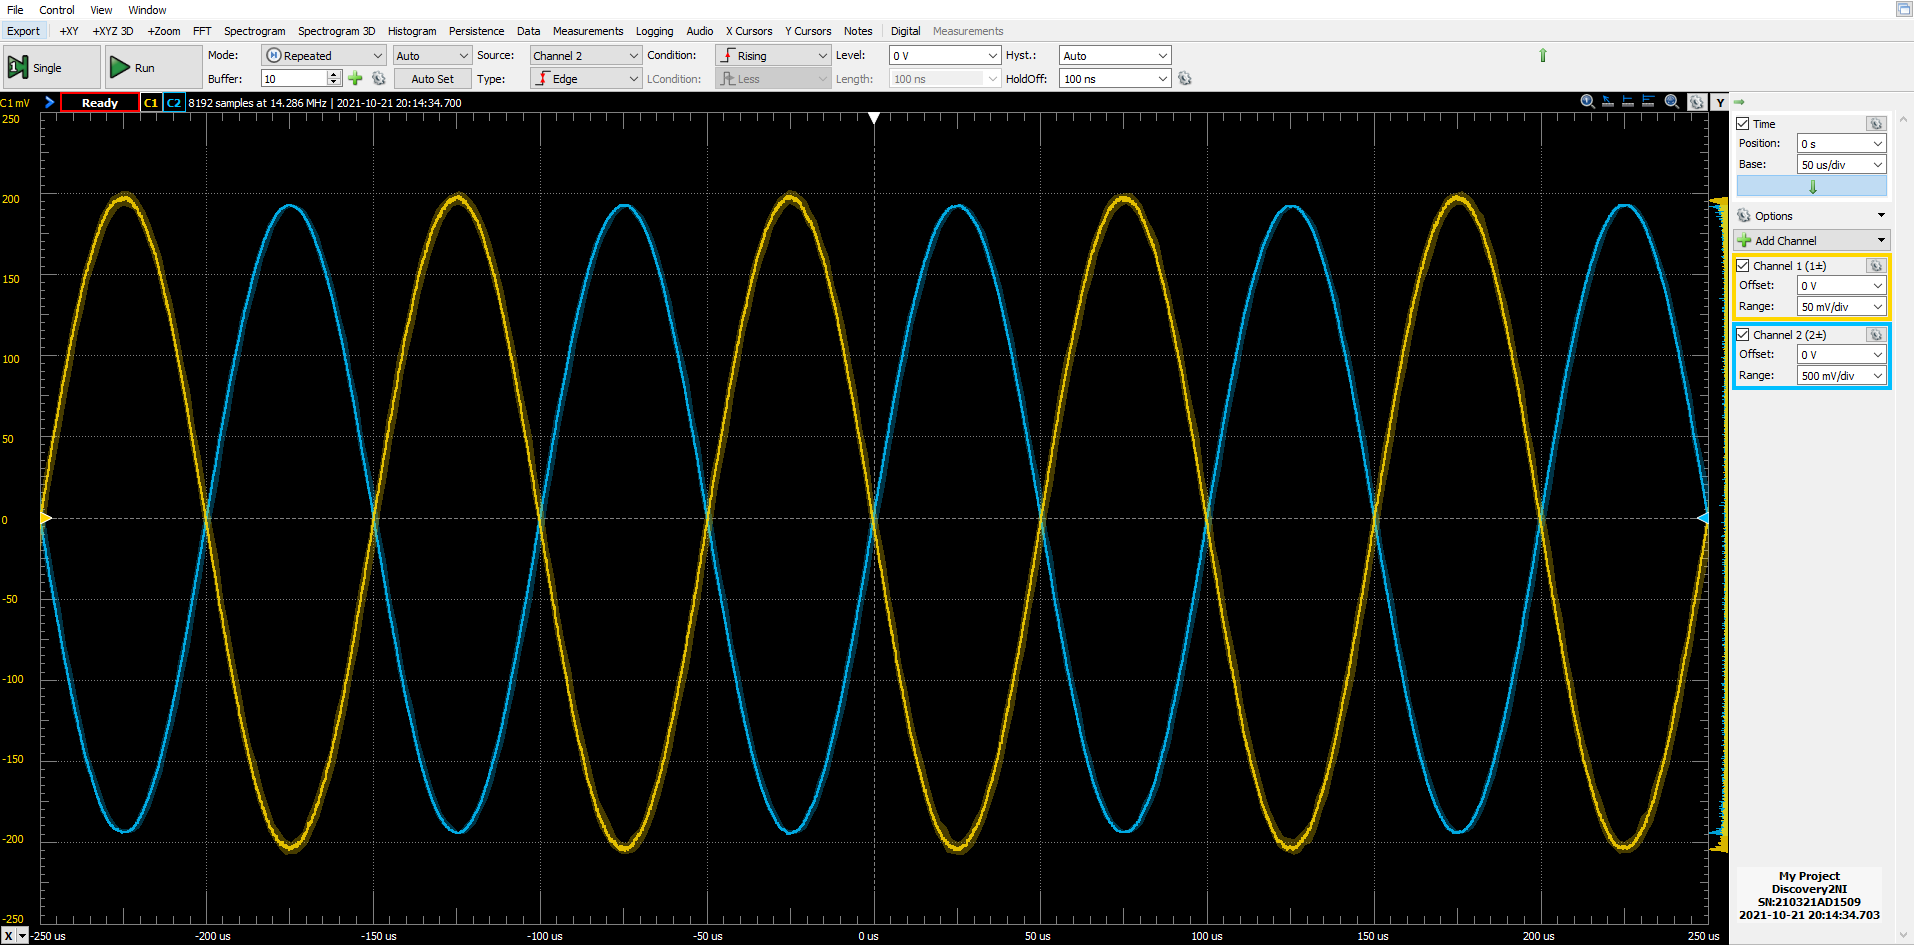
\includegraphics[scale=0.335]{Alin200mV}
\caption{Sovrapposizione dei plot di Bode ottenuti per l'amplificatore
non-invertente. \label{fig: prdbode}}
\end{figure}

\section*{Conclusioni e commenti finali}
Si è riusciti a costruire e studiare alcuni dei circuiti più comuni che si
possono realizzare con un amplificatore operazionale, tra cui: due filtri
attivi, passa-basso e passa-alto, un amplificatore di tensione invertente
(e uno non).
In particolare siamo riusciti ad apprezzare il differente comportamento dei
circuiti (anche in regime non lineare) dare una stima di guadagno, impedenza di
ingresso e frequenze caratteristiche della loro risposta in frequenza.

\section*{Dichiarazione}
I firmatari di questa relazione dichiarano che il contenuto della relazione \`e
originale, con misure effettuate dai membri del gruppo, e che tutti i firmatari
hanno contribuito alla elaborazione della relazione stessa.

\end{document}
